% =====================================================================
% TCC no formato SBC (modelo da Unit: tcc/modelo-tcc-sbc.tex)
% Compilar duas vezes: pdflatex tcc-afora-sbc.tex
% =====================================================================
\documentclass[a4paper,12pt]{article}

\usepackage[utf8]{inputenc}
\usepackage[T1]{fontenc}
% Português: com babel quando o pacote existe (TeX Live completo). Sem ele,
% os nomes são definidos à mão e a hifenização é desligada, para não hifenizar
% palavras portuguesas com padrões do inglês.
\IfFileExists{brazil.ldf}{\usepackage[brazilian]{babel}\newif\ifptbabel\ptbabeltrue}{%
  \newif\ifptbabel\ptbabelfalse}
\usepackage{microtype}
\usepackage{times}
\usepackage[a4paper,top=3.5cm,left=3cm,right=3cm,bottom=2.5cm]{geometry}
\usepackage{graphicx}
\usepackage{url}
\expandafter\def\expandafter\UrlBreaks\expandafter{\UrlBreaks\do\-}
\usepackage{indentfirst}
\usepackage{titlesec}
\usepackage[bf,sf,footnotesize,indent]{caption}
\usepackage{array}
\usepackage{tabularx}
\usepackage{booktabs}
\usepackage{listings}
\usepackage{xcolor}
\usepackage[authoryear,round,semicolon]{natbib}
% ABNT: \citep com o nome em maiúsculas; citações narrativas escritas como "Nome (\citeyear{chave})"
\providecommand{\NoCaseChange}[1]{#1} % TeX Live anterior a 2022 não define
\DeclareRobustCommand{\etal}{\NoCaseChange{\textit{et al.}}}
\makeatletter
\def\NAT@nmfmt#1{{\MakeUppercase{#1}}}
\makeatother

\setlength{\parindent}{1.27cm}
\setlength{\parskip}{6pt}
\raggedbottom

\titleformat{\section}{\fontsize{13}{15}\bfseries}{\thesection.}{1em}{}
\titleformat{\subsection}{\fontsize{12}{14}\bfseries}{\thesubsection.}{1em}{}
\titleformat{\subsubsection}{\fontsize{12}{14}\bfseries\itshape}{\thesubsubsection.}{1em}{}
\titlespacing*{\section}{0pt}{12pt}{6pt}
\titlespacing*{\subsection}{0pt}{10pt}{4pt}

\renewcommand{\captionfont}{\sffamily\footnotesize\bfseries}
\setlength{\captionmargin}{0.8cm}
\captionsetup{labelsep=period}
\captionsetup[table]{skip=4pt}

\newenvironment{resumo}{%
  \list{}{\advance\topsep by6pt\relax
    \leftmargin=0.8cm
    \labelwidth=0pt
    \listparindent=0pt
    \itemindent\listparindent
    \rightmargin\leftmargin}\item[\hskip\labelsep\bfseries\itshape Resumo.]\itshape}%
  {\endlist}

\renewenvironment{abstract}{%
  \list{}{\advance\topsep by6pt\relax
    \leftmargin=0.8cm
    \labelwidth=0pt
    \listparindent=0pt
    \itemindent\listparindent
    \rightmargin\leftmargin}\item[\hskip\labelsep\bfseries\itshape Abstract.]\itshape}%
  {\endlist}

% Listagens de código: legenda "Listagem N." acima, sem quebra de página
\renewcommand{\lstlistingname}{Listagem}
\lstdefinelanguage{TypeScript}{
  keywords={import,from,export,class,extends,const,private,public,static,return,new,get,void,string,implements,constructor,readonly,type},
  sensitive=true, comment=[l]{//}, morestring=[b]", morestring=[b]'}
\lstset{language=TypeScript, basicstyle=\ttfamily\footnotesize, columns=fullflexible,
  keepspaces=true, keywordstyle=\bfseries, commentstyle=\itshape\color{black!60},
  frame=lines, framesep=4pt, xleftmargin=6pt, xrightmargin=6pt,
  captionpos=t, abovecaptionskip=4pt, belowcaptionskip=4pt, upquote=true,
  literate={á}{{\'a}}1 {é}{{\'e}}1 {í}{{\'i}}1 {ó}{{\'o}}1 {ú}{{\'u}}1 {ç}{{\c{c}}}1 {ã}{{\~a}}1 {õ}{{\~o}}1 {ê}{{\^e}}1 {Ç}{{\c{C}}}1}

% Floats grandes (listagens) podem dividir a página com o texto
\renewcommand{\topfraction}{0.85}\renewcommand{\textfraction}{0.1}\renewcommand{\floatpagefraction}{0.8}

% Fonte de figuras e tabelas
\newcommand{\fonte}[1]{\par\vspace{2pt}{\centering\sffamily\footnotesize Fonte: #1\par}}
% Termos estrangeiros não dicionarizados
\newcommand{\estr}[1]{\textit{#1}}

\ifptbabel\else
  \renewcommand{\figurename}{Figura}\renewcommand{\tablename}{Tabela}
  \renewcommand{\refname}{Referências}\renewcommand{\contentsname}{Sumário}
  \hyphenpenalty=10000 \exhyphenpenalty=10000
  \emergencystretch=3em
\fi
\begin{document}
\pagestyle{empty}

\begin{center}
  {\fontsize{16}{20}\selectfont\bfseries Da cerimônia à declaração: o afora e as garantias de \textit{runtime} para \textit{backends} TypeScript escritos por pessoas e agentes de IA}\\[4pt]
  {\fontsize{14}{18}\selectfont\bfseries From ceremony to declaration: afora and runtime guarantees for TypeScript backends written by people and AI agents}\\[12pt]

  {\normalsize\bfseries Alan Reis Anjos$^{1}$, Luiz Gomes da Cunha Neto$^{1}$}\\[6pt]

  {\normalsize
    $^{1}$Ciência da Computação -- Universidade Tiradentes\\{}
    Aracaju, Sergipe -- SE\\{}
    \footnotesize\texttt{alanreisanjo@gmail.com, alan.reis@getafora.com, luiz\_gomes@unit.br}
  }
\end{center}
\vspace{6pt}
{\centering\footnotesize\itshape Relatório técnico: versão estendida do artigo de TCC de mesmo título, com os detalhes de medição, histórico e uso real que o artigo resume. Os \textit{scripts} e as saídas de \path{tcc/metrics/} estão em \url{https://github.com/Hoyasumii/tcc-afora}.\par}
\vspace{6pt}

\begin{resumo}
Agentes de IA barateiam a produção de código e encarecem a sua revisão; o conteúdo de baixa qualidade gerado em massa ganhou o nome de \textit{AI slop}. Este trabalho aplicado apresenta o afora, um \textit{framework} de código aberto para \textit{backends} em TypeScript, construído em três gerações segundo a Design Science Research. Quem escreve a aplicação, pessoa ou agente, declara o modelo do domínio, e o \textit{runtime} mantém invariantes genéricas: algumas por padrão, como a rejeição de campos não declarados e o mapeamento de erros, e outras a partir de declarações, como a unicidade e o controle de acesso. Um CRUD padrão coube em 3,6 vezes menos caracteres que uma versão enxuta em Hono e Zod; numa API real com regras próprias, porém, o código cresceu 27\% ao migrar para o afora e mudou de lugar. Numa avaliação de viabilidade, com uma execução por lado, um agente construiu um \textit{backend} só pelo servidor MCP do afora e manteve as cinco garantias verificadas sem código de implementação; a linha de base, escrita pelo mesmo agente em Hono e Zod, também as manteve. Construir entidades pequenas custou mais que validar com o Zod. Conclui-se que o afora preserva, por construção, as invariantes que declara; se isso reduz as falhas de agentes fica para uma avaliação em lote, já instrumentada.
\end{resumo}
\noindent\textbf{Palavras-chave:} \textit{AI slop}; agentes de IA; Domain-Driven Design; \textit{frameworks}; TypeScript.

\vspace{6pt}

\begin{abstract}
AI agents make code cheap to produce and expensive to review; the low-quality content they mass-produce has been named AI slop. This applied thesis presents afora, an open-source framework for TypeScript backends, built in three generations following Design Science Research. Whoever writes the application, person or agent, declares the domain model, and the runtime keeps generic invariants: some by default, such as rejecting undeclared fields and mapping errors, and others from declarations, such as unique keys and access control. A standard CRUD took 3.6 times fewer characters than a lean Hono and Zod version; in a real API with its own rules, however, the code grew 27\% when moved to afora, and changed place. In a feasibility evaluation with one run per side, an agent built a backend solely through afora's MCP server and kept the five checked guarantees with no implementation code; the baseline the same agent wrote in Hono and Zod kept them too. Building small entities cost more than validating with Zod. We conclude that afora preserves by construction the invariants it declares; whether this reduces agent failures is left to a batch evaluation that is already instrumented.
\end{abstract}
\noindent\textbf{Keywords:} AI slop; AI agents; Domain-Driven Design; frameworks; TypeScript.

\vspace{18pt}

% =====================================================================
\section{Introdução}

\subsection{Contexto}

Em fevereiro de 2025, Karpathy (\citeyear{karpathy2025}) chamou de \estr{vibe coding} a prática de pedir a um modelo de linguagem que escreva um programa e aceitar o resultado sem ler o código. Produzir software ficou muito mais barato, e produzir software ruim ficou mais barato ainda. O nome que se consolidou para o produto dessa segunda tendência é \estr{AI slop}: conteúdo gerado em quantidade por IA, sem cuidado, que custa a quem o recebe mais do que custou a quem o gerou. A Seção~\ref{sec:slop} reúne as evidências desse fenômeno no desenvolvimento de software.

\subsection{Problema}\label{sec:problema}

\estr{Backends} HTTP são um terreno especialmente fértil para esse tipo de falha. Um \estr{backend} correto precisa de garantias que não aparecem na especificação funcional: o \estr{hash} da senha não pode sair numa resposta, campos que o cliente não deveria enviar precisam ser recusados, um e-mail único não pode ser gravado duas vezes, um erro de negócio não pode virar HTTP~500, e um usuário não pode ler os dados de outro. Em \estr{frameworks} convencionais, cada uma dessas garantias é uma convenção: um \texttt{.strict()} num \estr{schema}, um filtro antes da resposta, uma checagem em cada rota. Convenções dependem de memória, e memória é justamente o que falha quando o código é escrito às pressas, por uma pessoa ou por um agente. O problema que este trabalho enfrenta é, portanto: \textbf{como projetar um \estr{framework} de \estr{backend} em que um conjunto de invariantes genéricas da API seja mantido pelo \estr{runtime}, e não pelo código da aplicação, e o que isso muda no que pessoas e agentes de IA precisam escrever e revisar?}

A resposta proposta tem dois níveis. Algumas garantias valem por padrão: não há linha da aplicação que as ligue, e por isso não há onde esquecê-las. Outras dependem de uma declaração, como dizer que um campo é único ou quem é o dono de um recurso; essas ainda podem ser esquecidas, mas num único lugar, o modelo, que se revisa lendo declarações e não implementações.

\subsection{Justificativa}\label{sec:justificativa}

A resposta usual ao \estr{AI slop} é revisar mais. Mas a revisão é o recurso escasso: quanto mais código um agente gera, mais caro fica confirmar que nenhuma garantia foi esquecida em nenhuma rota. Um \estr{framework} que tira essas garantias das mãos de quem escreve o código muda o objeto da revisão: em vez de procurar o que faltou em cada \estr{handler}, o revisor lê declarações. Há ainda uma justificativa de engenharia anterior à IA: arquiteturas como DDD e Clean Architecture exigem muito código repetitivo (\estr{boilerplate}), e código repetitivo é exatamente o tipo de código que se delega a agentes sem ler.

\subsection{Objetivos}\label{sec:objetivos}

O objetivo geral é desenvolver e avaliar um \estr{framework} para \estr{backends} em TypeScript que mantenha no \estr{runtime} um conjunto de invariantes de segurança e consistência de uma API, de modo que o código produzido por pessoas ou agentes de IA as preserve por construção, e medir o que isso muda no código que se escreve e se revisa.

Os objetivos específicos são:
\begin{enumerate}
  \item identificar, a partir da literatura e da experiência com duas gerações anteriores do artefato, as garantias que um \estr{backend} tende a perder quando escrito sem cuidado;
  \item projetar um modelo de declaração único (a \estr{blueprint}) do qual se derivem entidade, validação, repositório e contrato HTTP;
  \item implementar essas garantias como comportamento do \estr{runtime}, e não como \estr{plugins} ou convenções;
  \item oferecer a aplicação como dados (\texttt{afora.json}) e uma interface para agentes via Model Context Protocol (MCP);
  \item avaliar o produto quanto ao volume de código, à viabilidade de um \estr{backend} construído por agente que preserve as invariantes, ao custo de revisão e ao desempenho, e deixar instrumentada uma avaliação em lote que compare agentes com e sem o \estr{framework}.
\end{enumerate}

\subsection{Estrutura do trabalho}

A Seção~\ref{sec:fund} apresenta a fundamentação teórica, a análise de similares e os trabalhos relacionados; a Seção~\ref{sec:metodo}, a metodologia; a Seção~\ref{sec:desenv}, o desenvolvimento do produto, sua avaliação e a discussão dos resultados; e a Seção~\ref{sec:conclusao}, a conclusão.

% =====================================================================
\section{Fundamentação Teórica e Trabalhos Relacionados}\label{sec:fund}

\subsection{\textit{AI slop}: definição e manifestações}\label{sec:slop}

O uso de \estr{slop} para designar conteúdo ruim gerado por IA circulava em comunidades \estr{on-line} desde 2022, mas ganhou o debate público em maio de 2024, quando o programador Simon Willison propôs que \estr{slop} fosse para o conteúdo de IA indesejado o que \estr{spam} é para o e-mail indesejado \citep{willison2024}. Nem todo conteúdo gerado por IA é \estr{slop}, assim como nem toda mensagem promocional é \estr{spam}: o que o caracteriza é ser gerado sem cuidado e entregue a quem não o pediu nem o revisou. Uma formulação útil para este trabalho, atribuída a Neurotica e citada por Willison (\citeyear{willison2026}), define \estr{slop} como algo que exige mais esforço humano para consumir do que exigiu para produzir. Kommers \textit{et al.} (\citeyear{kommers2026}) observam que o termo ainda resiste a uma definição formal, o que não impediu sua adoção: em 2025, o Merriam-Webster o escolheu como palavra do ano \citep{merriam2025}.

A definição pela assimetria de esforço se estende ao trabalho. Pesquisadores do Stanford Social Media Lab e da BetterUp chamaram de \estr{workslop} o conteúdo gerado por IA que se parece com bom trabalho, mas não tem substância para avançar a tarefa; o efeito descrito é o de transferir o esforço de quem cria para quem recebe \citep{niederhoffer2025}.

No software, o caso mais documentado é o do curl. Em maio de 2025, o mantenedor Daniel Stenberg passou a banir quem enviasse relatórios de segurança considerados \estr{slop} \citep{newstack2026}; em julho, estimou que cerca de 20\% dos relatórios recebidos naquele ano eram \estr{slop} e que apenas cerca de 5\% apontavam vulnerabilidades reais \citep{stenberg2025}. Em janeiro de 2026, o projeto encerrou o programa de recompensas que mantinha desde 2019 \citep{stenberg2026}. O caso ilustra o mecanismo central do \estr{slop}: o custo de produzir caiu para quase zero, e o custo de verificar continuou humano.

\subsection{IA na engenharia de software}

Modelos de linguagem treinados em código passaram de completar funções isoladas \citep{chen2021} a resolver \estr{issues} reais de repositórios \citep{jimenez2024} e a operar como agentes que editam arquivos, executam comandos e usam ferramentas externas. O Model Context Protocol \citep{anthropic2024} padronizou a forma como esses agentes acessam ferramentas e dados, e é a interface pela qual o afora se oferece a eles.

Os efeitos sobre a produtividade são controversos, e os dois estudos mais citados ainda circulam como \estr{preprints}, sem revisão por pares. Um experimento controlado mediu tarefas 55,8\% mais rápidas com o GitHub Copilot \citep{peng2023}; um ensaio randomizado com 16 desenvolvedores experientes, em 246 tarefas de repositórios maduros, mediu tarefas 19\% mais lentas quando a IA era permitida, embora os participantes estimassem ter sido 20\% mais rápidos \citep{becker2025}. A diferença entre a velocidade percebida e a medida é o terreno onde o \estr{slop} prospera.

Os efeitos sobre a qualidade, nos estudos revisados por pares, são mais consistentes e negativos. Cerca de 40\% dos programas gerados pelo Copilot em cenários ligados a vulnerabilidades conhecidas eram vulneráveis \citep{pearce2022}. Em estudo com usuários, quem tinha acesso a um assistente escreveu código menos seguro na maioria das tarefas e se mostrou mais confiante de que ele era seguro \citep{perry2023}. O BaxBench, com 392 tarefas de geração de \estr{backends}, mostrou que o melhor modelo avaliado acertou a funcionalidade em apenas 62\% dos casos e que, em média, cerca de metade dos programas corretos de cada modelo podia ser explorada \citep{vero2025}. Modelos também recomendam pacotes que não existem \citep{spracklen2025}, o que abre espaço para que atacantes publiquem pacotes maliciosos com esses nomes (\estr{slopsquatting}). Como contexto, e não como evidência controlada, um relatório da indústria sobre 211 milhões de linhas alteradas entre 2020 e 2024 registrou aumento de blocos duplicados e queda de refatoração \citep{gitclear2025}. O traço comum é que o modelo produz código que parece correto, e o defeito está no que não aparece à primeira leitura; num \estr{backend}, isso significa as garantias implícitas descritas na Seção~\ref{sec:problema}.

\subsection{Domain-Driven Design e arquiteturas em camadas}

O Domain-Driven Design (DDD) propõe que o software seja estruturado em torno de um modelo do domínio, expresso numa linguagem ubíqua compartilhada entre desenvolvedores e especialistas \citep{evans2004}. Seus blocos táticos (entidades, objetos de valor, agregados, repositórios e serviços) foram detalhados por Vernon (\citeyear{vernon2013}). A Arquitetura Hexagonal \citep{cockburn2005} e a Clean Architecture \citep{martin2018} acrescentam uma regra de dependência: o domínio não conhece banco de dados, \estr{framework} web ou qualquer detalhe de infraestrutura, que se conecta a ele por portas e adaptadores.

O preço dessa separação é conhecido. Brooks (\citeyear{brooks1987}) distinguiu a complexidade essencial de um sistema, inerente ao problema, da complexidade acidental, introduzida pelas ferramentas e representações escolhidas. Em arquiteturas em camadas, boa parte do código de um recurso simples é acidental: classes de entidade, interfaces de repositório, casos de uso, fábricas, controladores e \estr{mappers} que repetem a mesma estrutura para cada novo conceito. Fowler (\citeyear{fowler2003}) descreve o risco oposto, o modelo de domínio anêmico, em que entidades viram contêineres de dados e a lógica se espalha por serviços. O afora tenta manter o modelo rico sem o custo da repetição.

\subsection{Engenharia dirigida por modelos e linguagens específicas de domínio}

A Engenharia Dirigida por Modelos (MDE) trata modelos como artefatos primários, a partir dos quais código e documentação são gerados \citep{schmidt2006,kleppe2003}. A programação generativa \citep{czarnecki2000} e as linguagens específicas de domínio, internas ou externas \citep{fowler2010,voelter2013}, reduzem a distância entre a intenção e a implementação. Uma crítica recorrente à MDE é o descompasso entre o modelo e o código gerado, que diverge ao primeiro ajuste manual \citep{hailpern2006}. O afora adota duas formas: uma DSL interna em TypeScript, para quem escreve código, e uma especificação em JSON, para quem gera código, com um caminho de ida e volta entre as duas.

\subsection{Validação em tempo de execução}

O sistema de tipos do TypeScript é estrutural e, por desenho, não existe após a compilação \citep{bierman2014}. Dados que chegam pela rede precisam, portanto, de validação em tempo de execução, o que deu origem a um ecossistema de bibliotecas de \estr{schema}, como Zod, Valibot, ArkType e TypeBox. O princípio \estr{parse, don't validate} \citep{king2019} propõe que a validação produza um valor de tipo mais preciso, em vez de apenas aceitar ou recusar a entrada. A especificação Standard Schema permite que ferramentas aceitem \estr{schemas} de qualquer biblioteca compatível \citep{standardschema2025}. O afora constrói suas propriedades sobre TypeBox e expõe cada uma como um Standard Schema.

\subsection{Segurança de APIs}

A OWASP API Security Top 10 \citep{owasp2023} lista os riscos mais frequentes em APIs. Quatro deles se relacionam com as garantias deste trabalho: a falha de autorização no nível do objeto (API1), em que um usuário acessa recursos de outro; a falha de autorização no nível da propriedade (API3), que reúne a exposição excessiva de dados e a atribuição em massa de campos que o cliente não deveria controlar; o consumo irrestrito de recursos (API4); e, em parte, a configuração de segurança incorreta (API8), que inclui mensagens de erro que expõem detalhes internos. A RFC 9457 \citep{rfc9457} padroniza o formato \path{application/problem+json} para respostas de erro, que o afora adota em todas as saídas HTTP.

\subsection{Análise de similares}\label{sec:similares}

Foram escolhidas quatro alternativas representativas do desenvolvimento de \estr{backends}: o NestJS, \estr{framework} TypeScript organizado em módulos, controladores e provedores; a combinação Hono + Zod, um servidor HTTP leve com uma biblioteca de \estr{schemas}, usada como linha de base na avaliação da Seção~\ref{sec:invariantes}; o tRPC, que compartilha tipos entre cliente e servidor sem um contrato HTTP explícito; e o Ruby on Rails, referência histórica de \estr{framework} opinativo baseado em convenção sobre configuração.

O critério de comparação não é o que cada ferramenta permite, mas o que ela garante por padrão, sem que o desenvolvedor escreva ou configure nada. Essa é a pergunta relevante quando o código é escrito por um agente que pode esquecer a configuração. A Tabela~\ref{tab:similares} resume a comparação.

\begin{table}[ht]
\centering
\caption{Garantias oferecidas por padrão pelas ferramentas analisadas.}\label{tab:similares}
\scriptsize
\renewcommand{\arraystretch}{1.15}
\begin{tabularx}{\linewidth}{>{\raggedright\arraybackslash}p{2.2cm}*{5}{>{\raggedright\arraybackslash}X}}
\toprule
Garantia & NestJS & Hono + Zod & tRPC & Rails & afora \\
\midrule
Campos não declarados recusados & Aceitos e atribuídos sem \texttt{Validation}\allowbreak\texttt{Pipe} e com ele no padrão; recusados (400) só com duas opções\textsuperscript{a,b} & Removidos por padrão; recusados (400) com \texttt{.strict()} e o \texttt{zValidator}, mas 500 sem ele nem um \texttt{onError}\textsuperscript{b} & Com Zod, removidos; recusados (400) com \texttt{z.strict}\allowbreak\texttt{Object}\textsuperscript{b} & Filtrados por \estr{strong parameters} em cada controlador & Recusados em qualquer profundidade (400) \\
Dados sensíveis fora das respostas & Vazam; ocultos só com \texttt{@Exclude} na classe e o interceptor\textsuperscript{b} & Manual\textsuperscript{b} & Manual\textsuperscript{b} & Manual (serializador ou \texttt{as\_json}) & Mascarados pelo \texttt{toJSON()}\textsuperscript{c} \\
Chaves únicas & Banco ou código da aplicação & Manual & Manual & Validação de modelo; sem índice único, sujeita a duplicatas & Garantidas pelo repositório (409)\textsuperscript{c} \\
Erro de negócio com o status correto & Exceções HTTP próprias; um \texttt{Error} comum vira 500\textsuperscript{b} & Manual (\texttt{onError})\textsuperscript{b} & Um \texttt{Error} comum vira 500 (\texttt{INTERNAL\_}\allowbreak\texttt{SERVER\_}\allowbreak\texttt{ERROR})\textsuperscript{b} & Parcial (alguns erros mapeados) & Por camada, em \texttt{problem+json} \\
Acesso por dono do recurso & \estr{Guards} escritos por rota & Manual & \estr{Middlewares} escritos & Manual por controlador & Declarado no caso de uso (\texttt{access}, \texttt{owner})\textsuperscript{c} \\
Aplicação descrita como dados para agentes & Não & Não & Não & Não & \texttt{afora.json} e servidor MCP \\
\bottomrule
\end{tabularx}
\fonte{elaborado pelo autor com base na documentação oficial consultada em novembro de 2026: NestJS~12, Hono~4.13, Zod~4.6, tRPC~11 e Rails~8.1 \citep{nestjs2026,zod2026,rails2026}. \textsuperscript{a}\texttt{whitelist} e \texttt{forbidNonWhitelisted} do \texttt{ValidationPipe}. \textsuperscript{b}Conferido com um projeto mínimo em 22/11/2026, no Bun~1.4.4: NestJS~12.6.0, tRPC~11.29.7 e Hono~4.13.20 (com e sem \texttt{@hono/zod-validator}~0.9.1), os dois últimos com Zod~4.6.7 (\path{tcc/metrics/similares/}). As células do Rails e as de chaves únicas e de acesso vêm só da documentação. \textsuperscript{c}No afora, vale para o que o modelo declara (\texttt{sensitive}, \texttt{unique}, \texttt{access}, \texttt{owner}); a senha (\texttt{ctx.password}) é sensível por padrão (Tabela~\ref{tab:garantias}).}
\end{table}

Duas ferramentas fora da tabela estão mais próximas da ideia de declarar o recurso e obter a API. O JHipster gera, para cada entidade descrita na sua linguagem JDL, uma entidade JPA, um repositório Spring Data, um controlador REST com o CRUD básico, as telas e os testes \citep{jhipster2026}; as garantias, porém, ficam no código gerado, que o desenvolvedor passa a manter e pode alterar. O PostgREST serve uma API REST a partir de um esquema PostgreSQL, autentica por JWT e delega a autorização aos papéis e às políticas de segurança por linha do próprio banco, o que seus autores descrevem como uma fonte declarativa única para a segurança \citep{postgrest2026}. É o precedente mais forte para a tese deste trabalho, com uma diferença de lugar: no PostgREST, o modelo e as garantias vivem no banco de dados; no afora, vivem no domínio em TypeScript, independentes do banco.

Os projetos mínimos usam o mesmo roteiro nas três ferramentas: um cadastro de usuário que devolve a entidade com o \estr{hash} da senha, uma requisição com a chave extra \texttt{isAdmin: true} e um e-mail repetido sinalizado por um \texttt{Error} comum. No NestJS, sem \texttt{ValidationPipe} e com ele na configuração padrão, a chave extra foi aceita e chegou à entidade; só com \texttt{whitelist} e \texttt{forbidNonWhitelisted} a requisição foi recusada com 400. O \estr{hash} saiu na resposta mesmo com o \texttt{ClassSerializerInterceptor} ligado, a não ser na classe marcada com \texttt{@Exclude}. No tRPC e no Hono, o \texttt{z.object} do Zod removeu a chave em silêncio. O \texttt{z.strictObject} a recusou com 400 no tRPC e, no Hono, com o validador idiomático \texttt{@hono/zod-validator}; sem ele e sem um \texttt{onError}, a recusa virou 500. Nas três, o erro comum virou 500. Nenhum desses comportamentos é defeito das ferramentas: cada um muda com uma linha de configuração ou de código, e é essa linha que um agente pode esquecer.

A tabela não diz que as alternativas sejam inseguras: um time disciplinado mantém todas essas garantias em qualquer uma delas. Ela diz onde mora a responsabilidade. Nas quatro primeiras colunas, a garantia vive no código da aplicação e precisa ser repetida em cada \estr{schema}, rota ou serializador; na última, vive no \estr{framework} e é escrita uma única vez, embora três delas ainda dependam de uma declaração no modelo (nota c). O Rails é o precedente mais próximo da filosofia do afora: suas convenções reduziram drasticamente o \estr{boilerplate} de aplicações web. A diferença está em que uma convenção ainda pode ser contrariada pelo código, enquanto uma garantia do \estr{runtime} não depende de quem escreve a aplicação conhecê-la.

\subsection{Trabalhos relacionados}\label{sec:relacionados}

A ideia de que o \estr{framework}, e não o desenvolvedor, deve carregar as defesas tem precedentes na literatura de segurança web. Finifter e Wagner (\citeyear{finifter2011}) compararam nove implementações da mesma aplicação web, em três linguagens, e concluíram que mecanismos de proteção automáticos do \estr{framework} (contra CSRF e na gestão de sessão) pareciam eficazes, enquanto mecanismos manuais pouco agregavam. Weinberger \textit{et al.} (\citeyear{weinberger2011}) analisaram a sanitização contra XSS em 14 \estr{frameworks} comerciais e encontraram uma distância grande entre as abstrações oferecidas e o que aplicações reais exigem: a automação só protege o que cobre. O trabalho mais próximo do afora é o GuardRails \citep{burket2011}, que anexa políticas de segurança, na forma de anotações, ao próprio modelo de dados de uma aplicação Rails e gera, por transformação de código-fonte, uma versão que as aplica automaticamente.

Do lado da medição, Vero \textit{et al.} (\citeyear{vero2025}) propõem um \estr{benchmark} que verifica, nos \estr{backends} gerados por LLMs, tanto a funcionalidade quanto a resistência a \estr{exploits}; é a forma de avaliação que a comparação entre agentes com e sem o afora pediria. Na geração de código por modelos de linguagem, a linha de pesquisa mais próxima restringe a saída do modelo durante a decodificação. O Synchromesh \citep{poesia2022} limita a amostragem a programas válidos na linguagem-alvo (SQL, Vega-Lite e SMCalFlow) e reduz erros de execução. Mündler \textit{et al.} (\citeyear{mundler2025}) estendem a restrição ao sistema de tipos, com uma formalização levada ao TypeScript, e reduzem os erros de compilação a menos da metade. Na modelagem, Cámara \textit{et al.} (\citeyear{camara2023}) avaliaram o ChatGPT em tarefas de UML e encontraram desempenho limitado, com deficiências sintáticas e semânticas e respostas inconsistentes, ao contrário do que se observa na geração de código.

\begin{table}[ht]
\centering
\caption{Posição do afora em relação aos trabalhos relacionados.}\label{tab:relacionados}
\scriptsize
\renewcommand{\arraystretch}{1.15}
\begin{tabularx}{\linewidth}{>{\raggedright\arraybackslash}p{2.6cm}>{\raggedright\arraybackslash}X>{\raggedright\arraybackslash}X}
\toprule
Trabalho & O que garante e onde & Relação com o afora \\
\midrule
Finifter e Wagner (\citeyear{finifter2011}) & Proteções automáticas do \estr{framework} superam as manuais (estudo empírico) & Sustenta o princípio de projeto; o afora estende a ideia a garantias de API \\
Weinberger \textit{et al.} (\citeyear{weinberger2011}) & Sanitização automática de XSS nos \estr{frameworks}, com lacunas & Alerta: a garantia só vale no que o \estr{framework} cobre (Seção~\ref{sec:limites}) \\
Burket \textit{et al.} (\citeyear{burket2011}) & Políticas anotadas no modelo de dados, aplicadas por transformação de código & Mesma direção (política no modelo); o afora aplica no \estr{runtime} e expõe o modelo a agentes \\
Vero \textit{et al.} (\citeyear{vero2025}) & Mede funcionalidade e segurança de \estr{backends} gerados por LLMs & Mede o problema sem propor proteção; um protocolo como o dele é o que falta à Seção~\ref{sec:invariantes} \\
Poesia \textit{et al.} (\citeyear{poesia2022}) & Saída do modelo restrita à gramática e à semântica de uma DSL, na decodificação & Restringe a geração; o afora restringe o que o código gerado pode violar \\
Mündler \textit{et al.} (\citeyear{mundler2025}) & Código bem tipado por decodificação restrita a tipos, em TypeScript & Complementar: tipos certos não impedem vazar um \estr{hash} \\
Cámara \textit{et al.} (\citeyear{camara2023}) & Limitações de LLMs em modelagem UML & Risco: o afora desloca o erro para o modelo, onde os LLMs são mais fracos \\
\bottomrule
\end{tabularx}
\fonte{elaborado pelo autor (2026).}
\end{table}

A Tabela~\ref{tab:relacionados} resume o posicionamento. Os trabalhos de decodificação restrita atuam antes do código existir, e só onde se controla o modelo de linguagem; o afora atua depois, sobre qualquer código, inclusive o escrito por uma pessoa ou por um agente fechado. Os dois enfoques se combinam. O trabalho de Cámara \textit{et al.} (\citeyear{camara2023}) aponta o custo da escolha do afora: se a garantia passa a depender de um modelo declarado corretamente, os erros de modelagem dos agentes ganham peso, e é ali que a revisão humana precisa se concentrar.

% =====================================================================
\section{Metodologia}\label{sec:metodo}

A pesquisa segue a Design Science Research (DSR), abordagem que produz conhecimento por meio da construção e da avaliação de artefatos que resolvem problemas relevantes \citep{hevner2004}. Hevner \textit{et al.} propõem sete diretrizes, entre elas que o artefato seja viável, que o problema seja relevante, que a avaliação seja rigorosa e que o projeto seja uma busca iterativa. Essa última descreve bem a história do produto: cada geração foi uma tentativa de solução, e sua avaliação definiu o problema da geração seguinte. Adota-se o processo de Peffers \textit{et al.} (\citeyear{peffers2007}), que organiza a DSR em seis atividades. A Tabela~\ref{tab:dsr} relaciona cada atividade ao que foi feito neste trabalho.

\begin{table}[ht]
\centering
\caption{Atividades da DSR e sua aplicação neste trabalho.}\label{tab:dsr}
\small
\renewcommand{\arraystretch}{1.15}
\begin{tabularx}{\linewidth}{>{\raggedright\arraybackslash}p{5.2cm}>{\raggedright\arraybackslash}X}
\toprule
Atividade \citep{peffers2007} & Neste trabalho \\
\midrule
1. Identificação do problema e motivação & Custo de \estr{boilerplate} no Roastery e garantias que dependem de convenção, agravadas pelo \estr{AI slop} (Seções~\ref{sec:problema} e~\ref{sec:fund}) \\
2. Definição dos objetivos da solução & Garantias no \estr{runtime}, declaração única do modelo, interface para agentes (Seção~\ref{sec:objetivos}) \\
3. Projeto e desenvolvimento & Três gerações: Caffeine, Roastery e afora (Seções 4.1 a 4.7) \\
4. Demonstração & Exemplos versionados (\path{examples/blog}, \path{examples/agent-built}) e dois sistemas em produção do autor: o CMS do \estr{site} do afora e a API do \estr{site} pessoal (Seção~\ref{sec:usoreal}) \\
5. Avaliação & Volume, invariantes, custo de revisão e desempenho (Seção 4.8) \\
6. Comunicação & Este trabalho, a documentação e o repositório público \\
\bottomrule
\end{tabularx}
\fonte{adaptado de Peffers \textit{et al.} (\citeyear{peffers2007}).}
\end{table}

Para desenhar a avaliação, adota-se o FEDS \citep{venable2016}, que classifica cada episódio de avaliação por dois eixos: a finalidade (formativa, para melhorar o artefato, ou somativa, para julgá-lo) e o paradigma (artificial, em ambiente controlado, ou naturalística, com usuários reais, problemas reais e sistemas reais). Neste trabalho, as avaliações de volume, invariantes, custo de revisão e desempenho são artificiais e somativas; o uso do afora em dois sistemas em produção (Seção~\ref{sec:usoreal}) é naturalístico, mas com um só usuário, o próprio autor. Não houve avaliação naturalística com usuários externos, e essa é a principal lacuna da estratégia.

Como o autor é também o desenvolvedor do artefato, a análise das gerações anteriores tem caráter de relato de experiência. Para limitar o viés, as afirmações se apoiam em evidências que terceiros podem verificar:
\begin{itemize}
  \item \textbf{Artefatos versionados}: os repositórios públicos do Roastery \citep{anjos2026roastery} e do afora \citep{anjos2026afora}, o histórico de \estr{commits} e o \texttt{CHANGELOG.md} do afora, que registra 16 versões publicadas entre 28 de outubro e 16 de novembro de 2026;
  \item \textbf{Volume}: o \estr{script} \path{tcc/metrics/count-volume.py} conta arquivos, linhas e caracteres não brancos de um mesmo CRUD em três formas, com o critério escrito no próprio \estr{script};
  \item \textbf{Invariantes}: a suíte \path{examples/agent-built}, que verifica seis invariantes sobre a API em execução, com controles negativos que mostram que cada verificação pode falhar;
  \item \textbf{Custo de revisão}: \path{tcc/metrics/review-cost.ts}, que conta as linhas e os caracteres dedicados a cada garantia na linha de base e no \texttt{afora.json}, a partir de uma classificação versionada e contestável;
  \item \textbf{Desempenho}: os \estr{benchmarks} versionados em \path{bench/}, executados em Bun e Node.js, e uma medição da requisição completa (\path{tcc/metrics/http-latency.ts}).
\end{itemize}

Os dados do afora referem-se à versão 27.0.0-rc.4, publicada em 16 de novembro de 2026, e ao \estr{commit} \texttt{cc1dbc2} do repositório. As medições de volume, custo de revisão e latência e a reexecução da avaliação de invariantes foram feitas em 19 de novembro de 2026, numa máquina virtual Linux x86-64 com 2 vCPUs (Intel Xeon a 2,1~GHz), 8~GB de memória, Bun~1.4.4 e Node.js~22.23; os \estr{benchmarks} de validação vêm do arquivo versionado \path{bench/results/latest.json}, gerado em 16 de novembro de 2026 numa máquina AMD EPYC 9V74 com Linux x86-64. Os comandos e as saídas estão em \path{tcc/metrics/}. Nenhuma medição usou a API de um modelo de linguagem.

% =====================================================================
\section{Desenvolvimento e Resultados}\label{sec:desenv}

\subsection{Histórico: três gerações de um artefato}

O afora não nasceu como \estr{framework}. Ele é a terceira geração de um projeto iniciado em janeiro de 2026, e cada geração foi, nos termos da DSR, um ciclo completo de projeto e avaliação. A Figura~\ref{fig:geracoes} resume a trajetória; as datas do Caffeine, do Roastery e da extração vêm do histórico de \estr{commits} dos repositórios da organização \texttt{roastery-cms}.

\begin{figure}[ht]
\centering
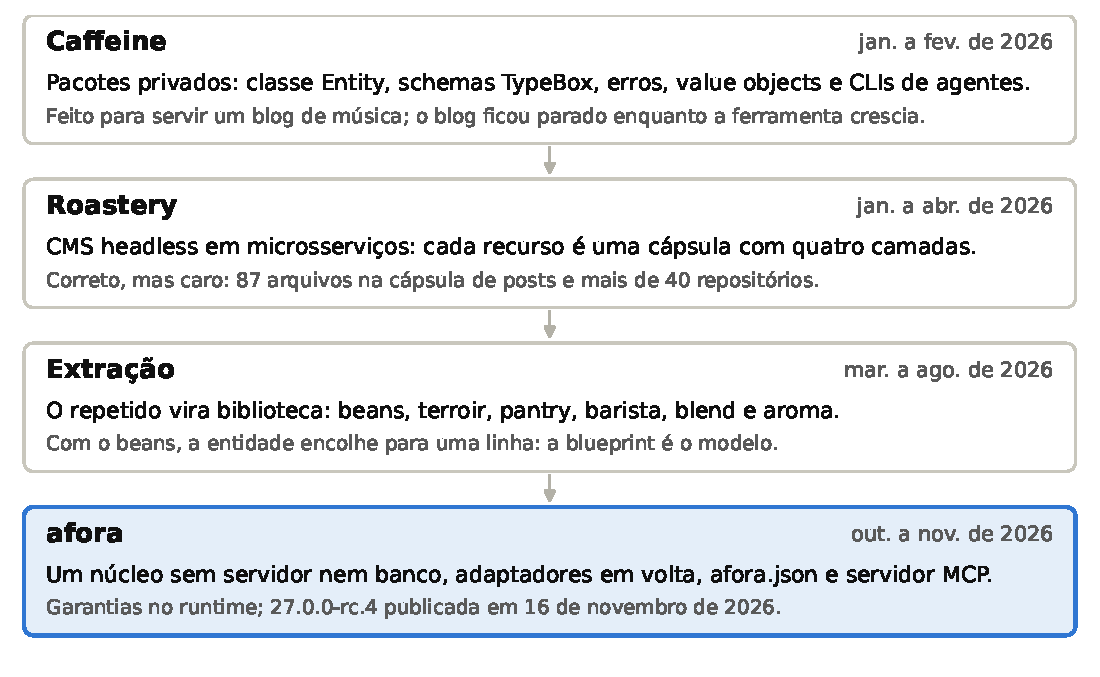
\includegraphics[width=.92\linewidth]{fig1.pdf}
\caption{As três gerações do artefato e a fase de extração.}\label{fig:geracoes}
\fonte{elaborado pelo autor (2026).}
\end{figure}

\textbf{Caffeine.} O ponto de partida foi um \estr{blog} de música, inspirado em publicações como Monkeybuzz, Música Instantânea e Angry Metal Guy. O protótipo tinha um problema: cada novo tipo de postagem exigia alterar o código, o que contrariava o propósito de ter um projeto de fim de semana sem abrir o terminal. A solução foi criar uma ferramenta: o Caffeine, um conjunto de pacotes privados com uma classe base \texttt{Entity} (que cuidava de \texttt{id}, \texttt{createdAt} e \texttt{updatedAt}), \estr{schemas} em TypeBox, uma família de erros, alguns \estr{value objects} e uma CLI para criar projetos. Ele também tinha pequenas CLIs para configurar agentes de IA em cada repositório, detalhe que, em retrospecto, antecipava a direção do produto final.

\textbf{Roastery.} O Caffeine virou o Roastery, um CMS \estr{headless} feito de microsserviços. Cada recurso (\estr{posts}, \estr{tags}, tipos de \estr{post}, modelos dinâmicos) era uma ``cápsula'': um pacote próprio, com as quatro camadas da Clean Architecture (domínio, aplicação, infraestrutura e apresentação), Prisma para o PostgreSQL, Redis para \estr{cache} e Elysia para HTTP. Funcionava e estava correto, mas era caro. A entidade \texttt{Post}, na Listagem~\ref{lst:roastery}, mostra o porquê.

\begin{lstlisting}[float=htbp,caption={Entidade \texttt{Post} da cápsula de \estr{posts} do Roastery (trecho).},label={lst:roastery}]
export class Post extends Entity<UnpackedPostSchema>
    implements IPost {
  private _name: DefinedStringVO;
  private _slug: SlugVO;
  private _description: DefinedStringVO;
  private _cover: UrlVO;

  private constructor(
    { cover, description, name, slug }: IConstructorPost,
    entityProps: EntityDTO,
  ) {
    super(entityProps);
    this._name = DefinedStringVO.make(
      name, this[EntityContext]("name"));
    this._slug = SlugVO.make(
      slug ?? name, this[EntityContext]("slug"));
    // ...o mesmo para description e cover
  }

  public static make(initialProps: IConstructorPost,
                     entityProps?: EntityDTO): IPost {
    return new Post(initialProps, entityProps ?? makeEntity());
  }

  @AutoUpdate
  rename(value: string): void {
    this._name = DefinedStringVO.make(
      value, this[EntityContext]("name"));
  }

  get name(): string { return this._name.value; }
  // ...um método e um getter por campo
}
\end{lstlisting}

Cada campo é escrito cinco vezes: o membro privado, o construtor, o método que o altera, o \estr{getter} e o \estr{schema}, que fica em outro arquivo. Em volta da entidade há interfaces de repositório, um caso de uso por operação, uma fábrica por caso de uso, um controlador por rota, um repositório Prisma, um repositório com \estr{cache} e os \estr{mappers} de cada um. O resto do custo estava fora do código: a organização passou de 40 repositórios, os adaptadores do Prisma eram submódulos Git, e mudar um pacote base significava publicá-lo e atualizar cada cápsula, uma por uma. Duas garantias, ocultar campos sensíveis das respostas e traduzir erros em status HTTP, eram responsabilidade de \estr{plugins} do servidor (um \estr{response mapper} e um \estr{error handler}) que funcionavam desde que alguém se lembrasse de ligá-los.

\textbf{Extração.} Entre março e agosto de 2026, o que se repetia em toda cápsula virou biblioteca: o \texttt{beans} (o modelo declarado uma vez, como um objeto simples, a \estr{blueprint}), o \texttt{terroir} (exceções que sabem a qual camada pertencem), o \texttt{pantry} (contratos de repositório por capacidade e casos de uso genéricos de CRUD), o \texttt{barista} (servidor HTTP com tratamento de erros e mapeamento de respostas), o \texttt{blend} (um manifesto em que a cápsula declara do que precisa) e o \texttt{aroma} (um \estr{logger} que serializa objetos de domínio de forma segura). Com o \texttt{beans}, a entidade acima encolheu para uma classe de uma linha sobre uma \estr{blueprint}. Foi ali que a ideia central ficou clara: a \estr{blueprint} é o modelo, e todo o resto pode ser derivado dela.

\textbf{afora.} As bibliotecas eram boas, mas continuavam sendo peças de um CMS, presas ao Elysia, ao Prisma e umas às outras, em vários repositórios. O afora é o resultado de consolidá-las: um núcleo só, sem dependência de servidor ou de banco, com pacotes em volta. A primeira versão publicada é de 28 de outubro de 2026, segundo o \texttt{CHANGELOG.md}; o código anterior a ela não tem histórico versionado. Quase todo conceito do afora tem um antepassado direto, como mostra a Tabela~\ref{tab:conceitos}.

\begin{table}[ht]
\centering
\caption{Conceitos do Roastery e seus correspondentes no afora.}\label{tab:conceitos}
\small
\renewcommand{\arraystretch}{1.15}
\begin{tabularx}{\linewidth}{>{\raggedright\arraybackslash}X>{\raggedright\arraybackslash}X}
\toprule
No Roastery & No afora \\
\midrule
A \estr{blueprint} do \texttt{beans}, \texttt{entityOf}, \estr{value objects} & \texttt{blueprintOf}, \texttt{entityOf}, as \estr{properties} padrão \\
As exceções por camada do \texttt{terroir} & \texttt{exceptionOf(\{ layer \})} e o rastro entre camadas \\
As interfaces de capacidade e o CRUD genérico do \texttt{pantry} & \texttt{repositoryOf(\{ actions \})} e os casos de uso padrão \\
O \texttt{barista} com \estr{error handler} e \estr{response mapper} & \texttt{outputOf}, \texttt{problem+json} e OpenAPI \\
O manifesto de cápsula do \texttt{blend} & \texttt{applicationOf} \\
A serialização segura do \texttt{aroma} & chaves \texttt{sensitive} mascaradas pelo \texttt{toJSON()} \\
As CLIs para agentes do Caffeine & \texttt{afora.json}, o servidor MCP e o gerador de código \\
\bottomrule
\end{tabularx}
\fonte{elaborado pelo autor (2026).}
\end{table}

A diferença entre as colunas não é de funcionalidade, mas de lugar: no Roastery, as garantias estavam em \estr{plugins} opcionais; no afora, estão no núcleo.

\subsection{Requisitos}

Os requisitos do afora foram derivados das falhas observadas no Roastery e das categorias de risco de APIs e de código gerado por IA discutidas na Seção~\ref{sec:fund}. A Tabela~\ref{tab:requisitos} lista os principais, separando funcionais (RF) de não funcionais (RNF), com a origem de cada um.

\begin{table}[ht]
\centering
\caption{Requisitos funcionais e não funcionais.}\label{tab:requisitos}
\small
\renewcommand{\arraystretch}{1.12}
\begin{tabularx}{\linewidth}{>{\raggedright\arraybackslash}p{0.10\linewidth}>{\raggedright\arraybackslash}p{0.52\linewidth}>{\raggedright\arraybackslash}X}
\toprule
Id & Requisito & Origem \\
\midrule
RF01 & Declarar uma entidade uma única vez e derivar dela validação, serialização, acessores e \estr{schema} & Repetição de campos no Roastery \\
RF02 & Mascarar propriedades sensíveis em qualquer serialização & \estr{Response mapper} opcional; OWASP API3 \\
RF03 & Rejeitar chaves não declaradas na entrada, em qualquer profundidade & Atribuição em massa; OWASP API3 \\
RF04 & Garantir chaves únicas no repositório, respondendo 409 & Integridade de dados \\
RF05 & Mapear exceções para status HTTP pela camada, em \texttt{problem+json} & \estr{Error handler} opcional; RFC 9457 \\
RF06 & Declarar acesso por escopo e por dono do recurso nos casos de uso & OWASP API1 \\
RF07 & Gerar documento OpenAPI a partir das declarações & Contrato HTTP explícito \\
RF08 & Descrever a aplicação em JSON e gerar o TypeScript correspondente & CLIs de agentes do Caffeine \\
RF09 & Expor a especificação e o gerador a agentes via MCP & Agentes como autores de código \\
RNF01 & Núcleo sem dependência de servidor HTTP ou banco de dados & Acoplamento ao Elysia e ao Prisma \\
RNF02 & Executar em Bun (1.4.4 ou superior) e Node.js (22 ou superior) & Portabilidade \\
RNF03 & Expor cada campo como Standard Schema & Interoperabilidade \\
RNF04 & Um contrato público único, com quebras apenas no \estr{major} anual & Mais de 40 repositórios sem matriz de versões \\
RNF05 & Medir o custo de validação e de construção de entidades em relação às bibliotecas de \estr{schema} mais usadas & Viabilidade em produção \\
\bottomrule
\end{tabularx}
\fonte{elaborado pelo autor (2026).}
\end{table}

\subsection{Arquitetura}

O afora é um monorrepositório em que um núcleo, \path{@afora/core}, concentra o modelo e as garantias, e pacotes independentes o ligam ao mundo exterior. A Figura~\ref{fig:arquitetura} mostra essa organização.

\begin{figure}[ht]
\centering
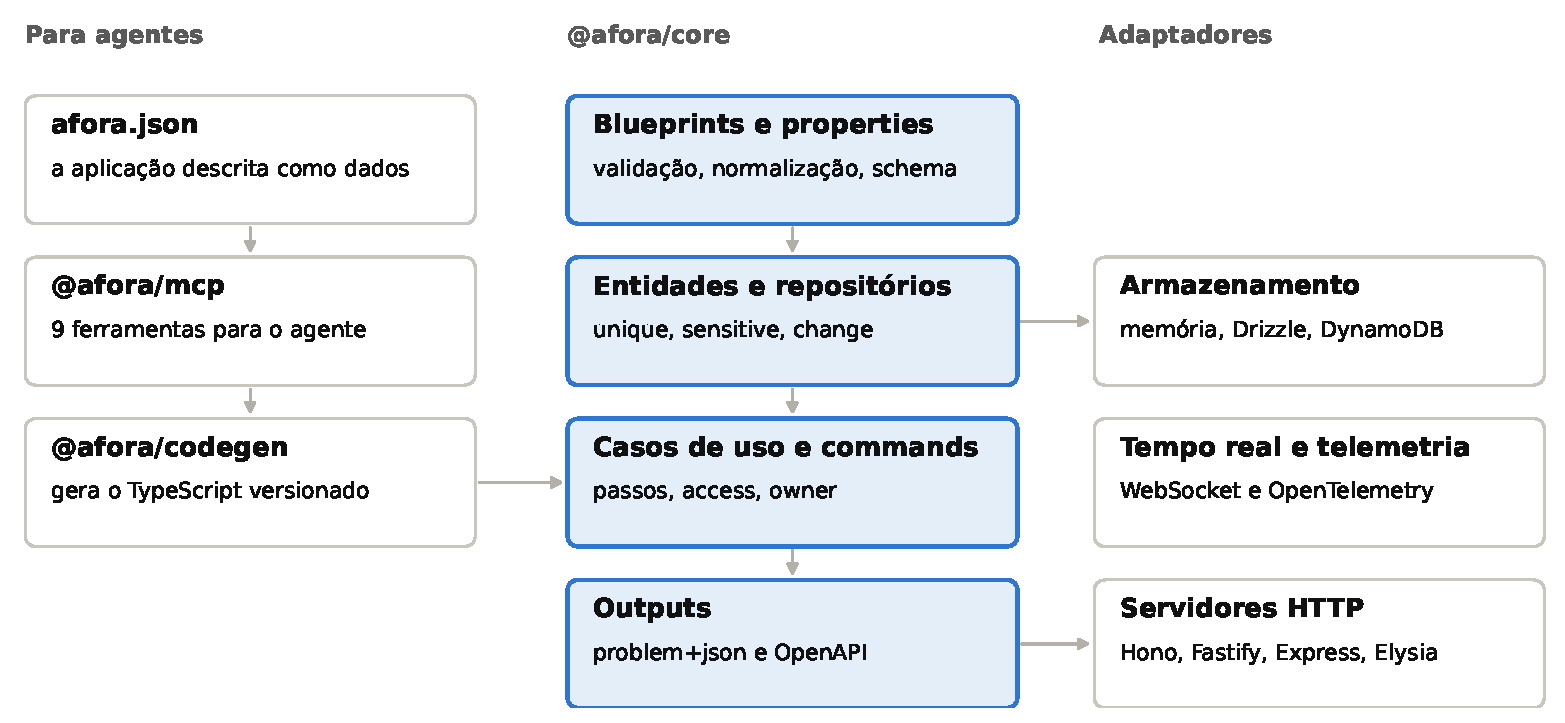
\includegraphics[width=\linewidth]{fig2.pdf}
\caption{Arquitetura do afora: núcleo, adaptadores e ferramentas para agentes.}\label{fig:arquitetura}
\fonte{elaborado pelo autor (2026).}
\end{figure}

A coluna central segue a progressão das camadas do DDD: \estr{blueprints} e \estr{properties} definem os valores; entidades e repositórios, o estado e sua persistência; casos de uso e \estr{commands}, as operações; e \estr{outputs}, a forma como essas operações são servidas. A regra de dependência da Clean Architecture é preservada: o núcleo não importa nenhum servidor ou banco, e cada adaptador implementa uma interface do núcleo (\texttt{IRepositoryProvider}, no caso do armazenamento, e um \estr{sink}, no caso dos servidores); o \path{@afora/otel} liga o rastreamento. Trocar Hono por Fastify, ou memória por Drizzle, não altera nenhuma declaração do domínio.

A coluna da esquerda é a contribuição específica para agentes. A especificação em \texttt{afora.json} é editada pelo servidor MCP e convertida pelo gerador em código que usa o núcleo exatamente como uma pessoa usaria. Não há um \estr{runtime} paralelo para código gerado: as garantias que valem para o código escrito à mão valem, pelo mesmo mecanismo, para o código escrito pelo agente.

\subsection{A \textit{blueprint} como modelo}

O afora parte de uma única premissa: a \estr{blueprint} é o modelo, e tudo o que pode ser derivado dela pertence ao \estr{framework}. A \estr{blueprint} é um objeto simples que associa cada campo a uma \estr{property}, um tipo de domínio com validação, normalização e \estr{schema} próprios. O mesmo \texttt{Post} da Listagem~\ref{lst:roastery} é declarado como na Listagem~\ref{lst:afora}.

\begin{lstlisting}[float=htbp,caption={O mesmo \texttt{Post} declarado no afora.},label={lst:afora}]
import { blueprintOf, entityOf } from "@afora/core";

class Post extends entityOf(
    blueprintOf((ctx) => ({
        name: ctx.text,        // sem espaços nas pontas, nunca vazio
        slug: ctx.slug,        // vira slug, e é chave única
        description: ctx.text,
        cover: ctx.url,
    })),
    { change: ["name", "slug", "description", "cover"] },
) {}
\end{lstlisting}

Dessa declaração saem o identificador, as datas de criação e atualização, os \estr{getters}, a validação, a forma JSON, o \estr{schema} OpenAPI e os métodos de alteração tipados (\texttt{post.change.name("...")}). Os tipos seguem o modelo: um repositório só oferece \texttt{findByEmail} se \texttt{email} for declarado único, e \texttt{user.change.password()} só existe se a alteração for permitida. Um agente que tenta chamar um método que o modelo não autoriza recebe um erro de compilação, e não um código que funciona por acaso.

As \estr{properties} padrão (\texttt{ctx.text}, \texttt{ctx.email}, \texttt{ctx.slug}, \texttt{ctx.url}, \texttt{ctx.password}, entre outras) carregam regras que um desenvolvedor apressado esqueceria: \texttt{email} é aparado e convertido para minúsculas; \texttt{password} só aceita um \estr{hash} argon2 e é sempre sensível; \texttt{url} recusa os protocolos \texttt{javascript:}, \texttt{data:}, \texttt{vbscript:} e \texttt{file:}.

\subsection{Garantias no \textit{runtime}}

A decisão de projeto mais importante foi mover para o \estr{runtime} garantias que, no Roastery, dependiam de \estr{plugins} configurados corretamente. A Tabela~\ref{tab:garantias} resume cada uma, como ela passa a valer e, quando houver, a categoria da OWASP API Security Top 10 \citep{owasp2023} relacionada.

A coluna ``Como vale'' separa dois tipos de garantia. As que valem \textbf{por padrão} não dependem de nenhuma linha da aplicação: um agente não tem como esquecê-las, só como contorná-las escrevendo código fora do caminho declarativo. As que valem \textbf{por declaração} são executadas pelo \estr{runtime}, mas só para o que o modelo declara: um campo marcado como \texttt{sensitive} ou \texttt{unique}, uma operação com \texttt{access} e \texttt{owner}. O \estr{framework} garante que a declaração será cumprida, não que ela será feita. O que muda em relação às alternativas é o lugar do esquecimento possível: uma linha do modelo, e não uma checagem em cada rota.

\begin{table}[ht]
\centering
\caption{Garantias mantidas pelo \textit{runtime} do afora.}\label{tab:garantias}
\footnotesize
\renewcommand{\arraystretch}{1.12}
\begin{tabularx}{\linewidth}{>{\raggedright\arraybackslash}p{0.2\linewidth}>{\raggedright\arraybackslash}X>{\raggedright\arraybackslash}p{0.17\linewidth}>{\raggedright\arraybackslash}p{0.2\linewidth}}
\toprule
Falha comum & Garantia no afora & Como vale & Risco relacionado \\
\midrule
\estr{Hash} de senha ou \estr{token} aparece numa resposta & Propriedades \texttt{sensitive} são mascaradas pelo \texttt{toJSON()} em qualquer profundidade & Por padrão em \texttt{ctx.password} (e na senha do \texttt{authenticatable}); por declaração (\texttt{sensitive}) nos demais & API3 (exposição excessiva de dados) \\
Campos extras no corpo são aceitos & Chaves não declaradas são rejeitadas em qualquer profundidade (400) & Por padrão & API3 (atribuição em massa) \\
Erro de negócio vira 500 & Exceções conhecem a própria camada e viram \texttt{problem+json} com o status correto & Por padrão; a camada de uma exceção própria é declarada & API8 (configuração de segurança incorreta, que inclui erros que expõem detalhes internos) \\
E-mail duplicado é gravado duas vezes & Chaves \texttt{unique} são garantidas pelo repositório (409) & Por padrão em \texttt{ctx.slug} e no e-mail do \estr{plugin} \texttt{authenticatable}; por declaração (\texttt{unique}) nos demais & Integridade de dados (fora do Top 10) \\
Um usuário lê ou altera dados de outro & Casos de uso declaram \texttt{access} (escopos, dono), verificado antes da execução & Por declaração (\texttt{access}, \texttt{owner}), em cada operação & API1 (autorização no nível do objeto) \\
Listagem sem limite & \texttt{list} rejeita (400) um \texttt{limit} acima de \texttt{maxLimit}, 100 por padrão & Por padrão & API4 (consumo irrestrito de recursos) \\
\bottomrule
\end{tabularx}
\fonte{elaborado pelo autor (2026), com base em OWASP (\citeyear{owasp2023}) e no código do afora (\path{src/std/properties/password.ts}, \path{src/std/use-cases/crud.ts}).}
\end{table}

As exceções merecem destaque. No afora, cada exceção declara a camada a que pertence (por exemplo, \texttt{Entity}, \texttt{UseCase} ou \texttt{Repository}) e carrega o rastro das camadas que atravessou. Erros internos são respondidos como 500 com o detalhe mascarado (exceto com a opção \texttt{debug} ativa), enquanto erros do cliente trazem a lista de problemas encontrados. O agente não precisa decidir o que pode ou não ser exposto: a camada decide.

\subsection{A aplicação como dados}

O afora foi desenhado para ser escrito também por agentes. Um arquivo \texttt{afora.json} declara entidades, casos de uso, \estr{commands} e a API HTTP. Casos de uso podem ser escritos como passos declarativos (\texttt{find}, \texttt{ensure}, \texttt{build}, \texttt{create}, \texttt{return}, entre outros), verificados pelo compilador quando \texttt{strictSteps} está ativo. O pacote \path{@afora/mcp} expõe um servidor MCP com nove ferramentas, entre elas \texttt{afora\_catalog} (o que o \estr{framework} oferece), \texttt{afora\_spec\_upsert} e \texttt{afora\_spec\_validate} (editar e validar a especificação) e \texttt{afora\_generate} (gerar o código e devolver os diagnósticos do TypeScript).

O \path{@afora/codegen} transforma a especificação no TypeScript que se escreveria à mão, versionado no repositório, e a função \texttt{extractSpec(app)} faz o caminho inverso. Isso endereça a crítica de Hailpern e Tarr (\citeyear{hailpern2006}) ao descompasso entre modelo e código: o que o agente produz é um \estr{diff} de declarações, e não de \estr{handlers}.

\subsection{Contrato, segurança e publicação}\label{sec:contrato}

Um \estr{framework} que promete garantias precisa ele próprio ser confiável. Três práticas sustentam isso:
\begin{itemize}
  \item \textbf{Contrato único.} As versões seguem o formato \texttt{AA.minor.patch}, em que o \estr{major} é o ano do ciclo; a partir da 27.0, uma quebra de compatibilidade só pode sair no \estr{major} do ano seguinte, após deprecação. Antes dela, as versões eram \texttt{0.0.x} e podiam quebrar a cada publicação; das 16 versões publicadas entre 28 de outubro e 16 de novembro de 2026, 12 são desse período (de 0.0.1 a 0.0.13, sem uma 0.0.10) e quatro são candidatas da 27.0. O salto de 0.0.13 para 27.0.0-rc.1 não é uma sequência de versões perdidas, mas a adoção desse esquema. Uma candidata (\estr{release candidate}) congela o contrato: durante ela, só entram correções, e a 27.0.0 sai quando não houver mais problemas bloqueantes abertos. Todo \estr{export} é registrado num \estr{snapshot}, e os tipos são testados em três versões do TypeScript.
  \item \textbf{Auditoria de segurança.} A versão 27.0.0-rc.3 corrigiu 19 achados de uma auditoria da rc.1; 17 deles têm um teste de regressão nomeado \texttt{SEC-<n>}, e os outros dois foram mudanças na integração contínua. Entre eles: \texttt{update} deixou de aceitar chaves sensíveis (uma senha poderia ser trocada por quem alcançasse a rota), a verificação de dono passou a comparar o valor já normalizado, e \texttt{login} passou a levar o mesmo tempo para e-mails existentes e inexistentes.
  \item \textbf{Cadeia de publicação.} A publicação no npm roda num \estr{job} isolado, com proveniência, sem \estr{scripts} de instalação e com todas as GitHub Actions fixadas por \estr{commit}; atualizações de dependências só são propostas após sete dias (exceto as de segurança), o que reduz a exposição a pacotes comprometidos.
\end{itemize}

\subsection{Avaliação}

A avaliação cobre quatro dimensões, cada uma ligada a um objetivo específico: o volume de código de um recurso (objetivo 2); a preservação de invariantes quando o código é escrito por um agente (objetivos 3 e 4); o custo de revisão, que sustenta a justificativa da Seção~\ref{sec:justificativa}; e o custo de desempenho da validação, medido conforme o RNF05 (objetivo 5). Uma quinta parte descreve o uso do afora em dois sistemas em produção.

\subsubsection{Volume de código}\label{sec:volume}

O mesmo CRUD de \estr{posts} foi contado em três formas, com o \estr{script} \path{tcc/metrics/count-volume.py}: (i) a cápsula \texttt{capsules.post\_post} do Roastery, no \estr{commit} \texttt{b0c4f1f} (27 de março de 2026); (ii) o afora, com as quatro declarações nomeadas (entidade, repositório, \estr{command} com as cinco operações e saída HTTP) e a aplicação que as liga, em \path{tcc/metrics/crud-afora/posts.ts}; e (iii) uma forma enxuta e convencional, em Hono, Zod e Drizzle sobre SQLite, sem DDD, em \path{tcc/metrics/crud-lean/posts.ts}. As formas (ii) e (iii) foram escritas para esta avaliação e têm o mesmo comportamento observável, conferido por um mesmo roteiro de requisições: criar, ler, listar, alterar e apagar; 401 sem \estr{token}; 400 com chave extra; 409 com \estr{slug} repetido; e 404 depois de apagar. Ambas deixam de fora as \estr{tags}, o \estr{cache} Redis e os repositórios remotos da cápsula; por isso, a Tabela~\ref{tab:volume} mostra a cápsula inteira e a cápsula sem essas partes.

\begin{table}[ht]
\centering
\caption{Volume de um mesmo CRUD de \textit{posts} em três formas.}\label{tab:volume}
\small
\renewcommand{\arraystretch}{1.12}
\begin{tabularx}{\linewidth}{>{\raggedright\arraybackslash}X rrrr}
\toprule
Forma & Arquivos & Linhas & Não vazias & Caracteres\textsuperscript{a} \\
\midrule
Roastery, cápsula inteira (\texttt{b0c4f1f}) & 87 & 2.335 & 2.052 & 59.994 \\
Roastery, sem \estr{cache}, repositórios remotos e dublês de teste & 77 & 1.806 & 1.631 & 47.843 \\
Hono + Zod + Drizzle, enxuto & 1 & 84 & 80 & 4.055 \\
afora (quatro declarações e a aplicação) & 1 & 52 & 47 & 1.122 \\
\bottomrule
\end{tabularx}
\fonte{elaborado pelo autor com \path{tcc/metrics/count-volume.py}; código de produção \texttt{.ts}, sem \texttt{*.spec.ts} e \texttt{*.test.ts}. \textsuperscript{a}Caracteres não brancos, medida que não depende da formatação.}
\end{table}

A forma (ii) usa o \texttt{resourceOf}, que declara as cinco operações padrão de uma vez; a comparação é, portanto, entre um recurso padrão declarado e um escrito à mão, e não entre duas formas de escrever código. Geradores de outros ecossistemas, como o \estr{scaffold} do Rails ou a CLI do NestJS, também produzem um CRUD com poucos comandos; a diferença é que deixam o código gerado no projeto, para ser mantido e revisado, enquanto o afora o mantém no \estr{framework}. Essa comparação não foi medida. A comparação que importa para o argumento não é com o Roastery, cuja arquitetura de microsserviços explica boa parte do volume, mas com a forma enxuta: em caracteres, o afora usa 3,6 vezes menos; em linhas, 1,6 vez menos, porque a versão enxuta foi escrita de forma compacta. A redução não elimina código: ela o desloca para o \estr{framework}. O núcleo do afora tem cerca de 39,5 mil linhas de TypeScript, sem os testes e contando comentários, e 104 arquivos de teste; o monorrepositório tem 174. O ganho está em escrever esse código uma vez, testá-lo uma vez, e não repeti-lo a cada recurso.

\subsubsection{Invariantes num \textit{backend} construído por agente}\label{sec:invariantes}

O exemplo \path{examples/agent-built} é uma avaliação de viabilidade: verifica se um agente que escreve um \estr{backend} apenas pelo servidor MCP chega a uma API que mantém as garantias do afora, já que nunca escreve o código que as mantém. A hipótese mais forte, de que agentes com o afora falham menos que sem ele, exige o lote descrito adiante e fica fora do que este trabalho mede.

\textbf{\textit{Briefings}.} O produto é um sistema de venda de ingressos: organizadores se cadastram e fazem \estr{login} para obter um \estr{token}, criam eventos com \estr{slug} único e capacidade, e vendem ingressos até esgotar. Há três versões do \estr{briefing}, com o mesmo contrato HTTP (rotas, corpos e status): a versão~1 não tem \estr{tokens} nem donos, e qualquer pessoa cria e lê qualquer evento; a versão~2 acrescenta o \estr{token} e eventos que só o seu organizador lê ou altera, e enuncia cada garantia como requisito de produto; a versão~3 descreve o mesmo produto e o mesmo contrato da versão~2, mas não lista as garantias (que a senha nunca aparece numa resposta, que campos desconhecidos são recusados, que nenhum erro vira 5xx), e é a que melhor testa a tese.

\textbf{Procedimento.} Para cada uma das versões 1 e 2, um agente de IA (Claude Opus 5.5, em sessões do Claude Code) produziu a especificação do afora; na versão~2, isso levou 26 chamadas de ferramenta. A especificação e o código de domínio foram produzidos apenas via MCP, sem edição manual; os únicos arquivos escritos à mão são o ponto de entrada do servidor e o catálogo de adaptadores. Um \estr{script} reproduz as chamadas num diretório vazio, e um teste confirma que o resultado é idêntico, byte a byte. A execução gravada, porém, não foi a primeira: como registra o \path{prompts.md} da execução, antes de gravar a mesma sessão já tinha escrito as verificações, ensaiado a especificação num diretório de rascunho e rodado contra ela as verificações de dono; as chamadas gravadas são a segunda passada. Como linha de base, a mesma sessão escreveu uma implementação em Hono + Zod a partir do mesmo \estr{briefing}. O repositório também contém um \estr{script} que faz $N$ execuções independentes por modelo, \estr{briefing}, banco e lado, com a API de modelos, e grava os \estr{prompts}, as chamadas e o resultado de cada execução. O lote não foi executado por falta de recursos para custear o uso da API: só a configuração mínima útil, com dez execuções por lado no \estr{briefing}~3, exige cerca de 330 requisições e 22 milhões de \estr{tokens} de entrada, segundo a estimativa do próprio \estr{script} (\texttt{--dry-run}), e este trabalho não teve financiamento. O protocolo, os \estr{scripts} e a estimativa estão versionados, e a execução é o primeiro trabalho futuro (Seção~\ref{sec:conclusao}). Uma execução manual do \estr{briefing}~3, como as das versões 1 e 2, também não foi feita: ela teria $n = 1$ e a mesma contaminação da linha de base descrita adiante.

\textbf{Verificações.} Um roteiro percorre o contrato HTTP sobre a API em execução, sem abrir porta, e verifica seis invariantes. As cinco primeiras correspondem às cinco primeiras linhas da Tabela~\ref{tab:garantias}; o limite de listagem (\texttt{maxLimit}) não é verificado por esta suíte, apenas pelos testes do núcleo. A sexta não é uma garantia do \estr{framework}, mas uma regra de negócio do \estr{briefing}, incluída para observar como cada lado a implementa: a capacidade sob compras simultâneas. Num evento de 3 lugares com 1 vendido, quatro compras são enviadas ao mesmo tempo para os 2 restantes; exatamente 2 devem ter sucesso, as outras devem receber \texttt{SoldOut} (422) em \texttt{problem+json}, e uma compra posterior também. A Tabela~\ref{tab:invariantes} mostra o resultado no \estr{briefing} 2; no \estr{briefing} 1, as cinco invariantes que se aplicam (todas menos a de dono) também passaram nos dois lados.

\begin{table}[ht]
\centering
\caption{Invariantes verificadas no \textit{backend} construído por agente (\textit{briefing} 2, uma execução por lado).}\label{tab:invariantes}
\small
\renewcommand{\arraystretch}{1.12}
\begin{tabularx}{\linewidth}{>{\raggedright\arraybackslash}X ccc}
\toprule
Invariante & Verificações & afora & Linha de base \\
\midrule
Nenhum valor sensível em respostas & 45 & 45/45 & 45/45 \\
Chaves não declaradas rejeitadas & 5 & 5/5 & 5/5 \\
Erros como \texttt{problem+json}, nunca 5xx & 21 & 21/21 & 21/21 \\
Chaves únicas garantidas & 2 & 2/2 & 2/2 \\
Apenas o organizador acessa seu evento & 12 & 12/12 & 12/12 \\
\midrule
\multicolumn{4}{l}{\textit{Regra de negócio, declarada pelo agente em passos (não é garantia do \textit{runtime})}} \\
Capacidade mantida sob compras simultâneas & 5 & 5/5 & 5/5 \\
\bottomrule
\end{tabularx}
\fonte{elaborado pelo autor a partir de \path{examples/agent-built/eval/RESULTS.md} \citep{anjos2026afora}, reexecutado em 19/11/2026 com \path{tcc/metrics/reeval.ts}, com o mesmo resultado.}
\end{table}

\textbf{Controles.} Para mostrar que cada invariante pode falhar, a mesma suíte é executada contra uma API deliberadamente descuidada (\estr{hash} na resposta, chaves desconhecidas aceitas, duplicatas permitidas, erros lançados, sem limite de capacidade), que falha em todas, e contra uma que verifica a capacidade e vende após um \texttt{await}, para mostrar que a verificação de concorrência detecta a condição de corrida.

\textbf{Resultado.} As duas implementações passaram em todas as verificações. Com uma execução por lado, a taxa de cada invariante é 1/1, cujo intervalo de Wilson a 95\% vai de 21\% a 100\%: o resultado mostra que o caminho funciona, não com que frequência. Ele também não distingue os lados, e portanto não confirma a hipótese de que o afora reduz falhas de agentes. Que o afora preserva as invariantes que declara é mostrado pela suíte de testes do repositório (174 arquivos) e pelos controles acima; o experimento acrescenta apenas que o mesmo vale para código produzido via MCP. A diferença observada está em como as garantias foram obtidas. No afora, nenhuma linha de implementação foi escrita para as cinco primeiras, mas elas ocupam 82 linhas de declaração no \texttt{afora.json} (Tabela~\ref{tab:revisao}), que também se revisam e também podem estar erradas: a especificação declara um organizador autenticável, um \estr{slug}, as exceções e seus status, e um \texttt{access} com \texttt{owner} em cada operação de evento. A sexta não é gratuita: o agente a declarou em passos na especificação (carregar o evento, gravar o ingresso, perguntar ao repositório se existe ingresso além da capacidade e lançar \texttt{SoldOut} se existir), e a transação do \estr{command} desfaz o ingresso excedente. A linha de base, escrita pelo agente sem o \estr{framework}, implementou cada garantia no próprio código: \texttt{.strict()} em cada \estr{schema} Zod, uma função que remove o \estr{hash} antes de cada resposta, tratamento próprio de erros em \texttt{problem+json}, mapas próprios para e-mails e \estr{slugs} únicos, assinatura e verificação de \estr{token}, uma checagem de dono em cada rota de evento e um contador de capacidade.

\textbf{Concorrência.} As execuções versionadas usam armazenamento em memória; nenhuma execução em SQLite foi feita por agente. Com um armazenamento síncrono (um \estr{array} em JavaScript, ou o \texttt{bun:sqlite}, cujas chamadas não cedem a vez), uma leitura e uma escrita sem \texttt{await} entre elas não se intercalam, e a verificação tende a passar nos dois lados: ela só reprova uma implementação que espera entre ler a contagem e gravar o ingresso, ou que não verifica a capacidade. Neste experimento, portanto, a sexta invariante não separa o afora da linha de base.

\subsubsection{Custo de revisão}\label{sec:revisao}

A justificativa da Seção~\ref{sec:justificativa} afirma que, no afora, o revisor lê declarações em vez de implementações. Para medir o tamanho do que se revisa, cada linha da linha de base (\path{baseline/runs/claude-code-2/app.ts}) e do \texttt{afora.json} do \estr{briefing} 2 foi atribuída a uma garantia, ou a nenhuma. A classificação está em \path{tcc/metrics/review-cost.classes.json}, com faixas de linhas que qualquer pessoa pode contestar. O \texttt{afora.json} é formatado pelo servidor MCP com um valor por linha, o que infla a contagem de linhas; por isso a Tabela~\ref{tab:revisao} também traz os caracteres não brancos.

\begin{table}[ht]
\centering
\caption{Linhas e caracteres dedicados a cada garantia na linha de base e no \texttt{afora.json} (\textit{briefing} 2).}\label{tab:revisao}
\small
\renewcommand{\arraystretch}{1.12}
\begin{tabularx}{\linewidth}{>{\raggedright\arraybackslash}X rrrr}
\toprule
 & \multicolumn{2}{c}{Linha de base (Hono + Zod)} & \multicolumn{2}{c}{afora (\texttt{afora.json})} \\
Garantia & Linhas & Caracteres & Linhas & Caracteres \\
\midrule
Chaves não declaradas & 5 & 50 & 0 & 0 \\
Valores sensíveis & 4 & 168 & 3 & 29 \\
Erros em \texttt{problem+json} & 58 & 1.285 & 28 & 479 \\
Chaves únicas & 18 & 379 & 1 & 14 \\
\estr{Token} e dono & 55 & 1.587 & 50 & 500 \\
Capacidade & 6 & 201 & 19 & 204 \\
\midrule
Total das garantias & 146 & 3.670 & 101 & 1.226 \\
Arquivo inteiro & 283 & 7.358 & 357 & 4.491 \\
\bottomrule
\end{tabularx}
\fonte{elaborado pelo autor com \path{tcc/metrics/review-cost.ts} e \texttt{review-cost-chars.py}; linhas não vazias.}
\end{table}

O resultado é mais modesto que a tese sugeria. Em caracteres, as garantias ocupam três vezes menos no afora (1.226 contra 3.670), e quatro delas quase desaparecem. Mas a garantia de dono e de \estr{token}, a mais importante para a OWASP, ocupa quase o mesmo número de linhas nos dois lados (50 contra 55), porque o \texttt{afora.json} repete o \texttt{access} e o \texttt{owner} em cada operação; e a capacidade custa mais no afora, porque foi declarada em passos. Em linhas, o \texttt{afora.json} inteiro é maior que a linha de base. A diferença que a tabela não capta é de natureza: as linhas do afora dizem quem é o dono, e as da linha de base implementam a verificação (extrair o \estr{token}, verificar a assinatura, comparar o dono), e cada uma pode estar errada. O tempo efetivo de revisão não foi medido.

\subsubsection{Desempenho}\label{sec:desempenho}

Garantias no \estr{runtime} têm um custo. Como o afora normaliza os valores, coleta todos os erros e devolve um novo valor, ele faz mais trabalho por validação que verificadores puros. Os \estr{benchmarks} versionados comparam o afora com nove bibliotecas em sete cenários, exigindo que todas declarem as mesmas regras e rejeitem chaves não declaradas. A Tabela~\ref{tab:bench} traz três cenários nos três \estr{runtimes} medidos, com dois caminhos do afora: \texttt{blueprint.safeParse}, que só valida, e \texttt{Entity.safeParse}, que constrói a entidade e é o caminho real de uma requisição.

\begin{table}[ht]
\centering
\caption{Mediana do tempo de validação, em nanossegundos (menor é melhor).}\label{tab:bench}
\scriptsize
\renewcommand{\arraystretch}{1.12}
\begin{tabularx}{\linewidth}{>{\raggedright\arraybackslash}p{1.9cm}>{\raggedright\arraybackslash}X rrrrr}
\toprule
\estr{Runtime} & Cenário (entrada válida) & afora \texttt{blueprint} & afora \texttt{Entity} & Zod~4 & Valibot & TypeBox compilado \\
\midrule
Bun 1.4.4 & objeto pequeno & 229 & 836 & 446 & 240 & 44 \\
 & \estr{payload} de API & 1.714 & 3.197 & 4.395 & 2.311 & 702 \\
 & sem transformação & 87 & 603 & 273 & 147 & 44 \\
\addlinespace
Node.js 22.23 & objeto pequeno & 309 & 1.422 & 525 & 410 & 63 \\
 & \estr{payload} de API & 2.488 & 4.807 & 4.523 & 4.302 & 1.048 \\
 & sem transformação & 158 & 1.217 & 220 & 282 & 67 \\
\addlinespace
Node.js 24.22 & objeto pequeno & 315 & 1.398 & 518 & 876 & 64 \\
 & \estr{payload} de API & 2.456 & 3.907 & 4.407 & 4.133 & 1.059 \\
 & sem transformação & 178 & 1.199 & 210 & 729 & 64 \\
\bottomrule
\end{tabularx}
\fonte{\path{bench/results/latest.json} (afora 27.0.0-rc.4, \estr{commit} \texttt{82e24ea}, AMD EPYC 9V74, Linux x86-64, 16/11/2026), resumido por \path{tcc/metrics/bench-summary.py}; os sete cenários, as entradas inválidas e as demais bibliotecas estão na saída do \estr{script}.}
\end{table}

A validação pura do afora é comparável à das bibliotecas mais usadas e, na maioria dos cenários, mais rápida que a do Zod; o TypeBox compilado, que apenas verifica sem transformar, leva de um quinto à metade do tempo do afora nos cenários da Tabela~\ref{tab:bench}. O afora perde no caminho real: \texttt{Entity.safeParse} leva de 1,9 a 2,7 vezes o tempo do Zod para um objeto pequeno, e de 2,2 a 5,7 vezes no cenário sem transformação, nos três \estr{runtimes}. Nos \estr{payloads} de API maiores, ele volta a ficar à frente do Zod no Bun e no Node.js~24 e empata no Node.js~22. Como o RNF05 não fixou de antemão um limite aceitável, este trabalho não declara o requisito cumprido ou descumprido: relata que a validação pura fica na faixa das bibliotecas mais usadas e que a construção de entidades pequenas custa várias vezes mais. Limites desse tipo existem no repositório, verificados na integração contínua como razão em relação ao Zod (\path{bench/guard.limits.ts}): 1,15 vez para \texttt{blueprint.safeParse} e 2 vezes para \texttt{Entity.safeParse}, com exceções justificadas por cenário. Eles servem para detectar regressões e foram calibrados a partir das próprias medições, e não fixados antes delas.

Para pôr esses números em escala, a requisição inteira foi medida dentro do processo, sem rede, nos dois CRUDs da Seção~\ref{sec:volume} (\path{tcc/metrics/http-latency.ts}, Bun~1.4.4, mediana após 200 requisições de aquecimento). Cada medição foi repetida dez vezes, em processos separados, para 300, 1.000 e 3.000 registros (\path{http-latency-rep.ts}). A mediana das dez execuções foi de 252 a 488~µs para criar um \estr{post} no afora, contra 125 a 164~µs na forma enxuta, e de 203 a 449~µs para lê-lo, contra 66 a 98~µs. Em razão, o afora levou 1,6, 2,0 e 3,7 vezes o tempo da forma enxuta para criar, e 2,2, 3,2 e 6,3 vezes para ler, nos três tamanhos; os intervalos interquartis das razões ficaram entre 1,3 e 7,8. O tempo do afora cresce com o número de registros por causa do provedor em memória, feito para desenvolvimento e testes: a verificação de unicidade percorre todos os registros da tabela, e cada transação copia as tabelas (\path{src/core/repository/in-memory.ts}). A forma enxuta usa SQLite em memória, de modo que a comparação mistura o custo do \estr{framework} com o do armazenamento. Com 3.000 registros, a mediana de algumas execuções do afora passou de meio milissegundo (até 612~µs). A relação desse custo com a latência de rede e de banco de um \estr{backend} real não foi medida.

\subsubsection{Uso em sistemas reais}\label{sec:usoreal}

As avaliações anteriores são artificiais, no sentido do FEDS \citep{venable2016}. Para observar o afora fora de um experimento, esta seção descreve dois sistemas em produção que o usam, ambos do próprio autor e escritos em grande parte com agentes. Eles não substituem uma avaliação com usuários externos, mas mostram o artefato diante de requisitos que ninguém escolheu para favorecê-lo: armazenamentos próprios, autenticação de terceiros, \estr{upload} de arquivos e um servidor MCP. Os números vêm de \path{tcc/metrics/real-use.sh}, com o mesmo critério de linhas não vazias da Seção~\ref{sec:volume}.

\textbf{O CMS do \estr{site} do afora.} O \estr{blog}, as notícias e o livro do \texttt{getafora.com} são servidos por um CMS \estr{headless} cujo domínio é escrito com o \path{@afora/core} na versão 0.0.11, anterior à auditoria de segurança da rc.3 (Seção~\ref{sec:contrato}). A API roda no AWS Lambda sobre o DynamoDB, com um provedor de armazenamento próprio, e o painel administrativo é uma aplicação React. No \estr{commit} \texttt{78b772f}, o domínio e a API somam 138 arquivos e 21.461 linhas não vazias, com 10 entidades, 10 repositórios, 37 casos de uso e 43 exceções declarados, e 46 arquivos de teste; dos 167 \estr{commits} (8 a 16 de novembro de 2026), 119 têm coautoria de um modelo Claude. O sistema usa o núcleo (entidades com chaves sensíveis, como o \estr{hash} dos \estr{tokens} de API; exceções por camada; repositórios), mas não a saída HTTP do afora: as rotas são escritas em Hono, o mapeamento de exceções para status é uma função própria, e as respostas da API administrativa são montadas campo a campo. Nesse sistema, portanto, três das garantias da Tabela~\ref{tab:garantias} voltam a ser código da aplicação.

\textbf{A API do \estr{site} pessoal.} O \estr{site} \texttt{hoyasumii.dev} tem um painel de conteúdo e uma API no Cloudflare Workers sobre o Supabase, em repositório público \citep{anjos2026site}. Em 11 de novembro de 2026, a API, que era escrita em Hono puro, foi refeita sobre o \path{@afora/core} e o \path{@afora/hono} (\estr{commit} \texttt{4f41cb3}); a mudança entrou no ramo principal em 16 de novembro, já na versão 27.0.0-rc.2. Todas as 21 alterações da API têm coautoria do Claude Opus 5.5. A Tabela~\ref{tab:usoreal} compara o código antes e depois.

\begin{table}[ht]
\centering
\caption{Linhas não vazias da API do \textit{site} pessoal antes e depois da migração para o afora.}\label{tab:usoreal}
\small
\renewcommand{\arraystretch}{1.12}
\begin{tabularx}{\linewidth}{>{\raggedright\arraybackslash}X rr}
\toprule
Parte & Antes (Hono puro) & Depois (afora) \\
\midrule
Serviços (regras e operações) & 703 & 113 \\
Repositórios & 432 & -- \\
Rotas & 465 & 300 \\
Domínio afora (entidades, casos de uso, saída) & -- & 1.544 \\
Provedor do Supabase & -- & 314 \\
Contrato compartilhado (\path{schema.ts}) & 351 & 481 \\
Demais arquivos & 1.393 & 1.480 \\
\midrule
Total (\path{apps/api/src} e \path{packages/shared/src}) & 3.344 & 4.232 \\
\bottomrule
\end{tabularx}
\fonte{elaborado pelo autor com \path{tcc/metrics/real-use.sh}, no repositório \texttt{Hoyasumii/Hoyasumii} (\estr{commits} \texttt{4f41cb3\^{}} e \texttt{4f41cb3}); código \texttt{.ts}, sem testes.}
\end{table}

O código cresceu 27\%. A redução da Tabela~\ref{tab:volume} não se repetiu porque o caso é outro: lá, um CRUD padrão escrito em \texttt{afora.json}; aqui, casos de uso com regras próprias, escritos à mão com a API em TypeScript, e um provedor de armazenamento que o afora não tinha. O que mudou foi o lugar do código: repositórios e serviços escritos à mão deram lugar a declarações, e a validação, a recusa de chaves e o \texttt{problem+json} passaram a vir da saída HTTP do afora, exceto em quatro rotas que continuam em Hono puro (saúde, \estr{upload} \estr{multipart}, MCP e OAuth).

A revisão feita depois da migração (\estr{commit} \texttt{c9b5172}) mostra o limite da tese num caso real. Entre os defeitos corrigidos, a verificação de unicidade do provedor do Supabase olhava só a primeira linha que tinha o valor. A unicidade é uma garantia do afora, mas quem a executa é o provedor, e um provedor escrito pela aplicação é código da aplicação. O afora oferece um kit de contrato para provedores (\texttt{providerContract}), que o projeto usa; no entanto, ele só roda com um Supabase local, e o defeito foi encontrado na revisão, não por ele.

\subsection{Discussão}

\subsubsection{O afora diante do \textit{AI slop}}

O argumento deste trabalho pode ser resumido assim: o \estr{AI slop} em software resulta de uma assimetria entre o custo de gerar e o de verificar, e \estr{frameworks} podem reduzir essa assimetria diminuindo o que precisa ser verificado. Os resultados sustentam parte do argumento; a parte que dependeria de comparar agentes com e sem o \estr{framework} não foi medida.

\textbf{Reduz a superfície de erro.} Se uma garantia vive no \estr{runtime} e vale por padrão, não há linha da aplicação em que ela possa ser esquecida; se depende de uma declaração, pode ser esquecida num só lugar (Tabela~\ref{tab:garantias}). Os estudos de Pearce \textit{et al.} (\citeyear{pearce2022}) e Perry \textit{et al.} (\citeyear{perry2023}) mostram que assistentes tendem a produzir código vulnerável com aparência de correto, e Finifter e Wagner (\citeyear{finifter2011}) mostram que proteções automáticas do \estr{framework} funcionam onde as manuais falham. No experimento, o afora manteve as cinco garantias genéricas sem uma linha de implementação, com 82 linhas de declaração; a linha de base precisou de 140 linhas de código para as mesmas cinco (146 com a capacidade). O que o experimento não mostra é que um agente sem o afora as esqueceria: na única execução, ele não esqueceu.

\textbf{Torna a revisão menor, mas não pela metade.} Se o \estr{slop} é o que custa mais para consumir que para produzir (Seção~\ref{sec:slop}), a saída é baratear o consumo. A Tabela~\ref{tab:revisao} mostra que o texto dedicado às garantias encolhe três vezes em caracteres, mas que a autorização continua exigindo uma declaração por operação, que o revisor precisa ler. A pergunta do revisor muda de ``o que foi esquecido em cada \estr{handler}?'' para ``o modelo e as declarações estão certos?'', que é uma pergunta sobre o domínio, e não sobre a infraestrutura; se isso é mais rápido de responder não foi medido.

\textbf{Reduz a repetição.} No afora, o código que seria duplicado (construtores, \estr{getters}, \estr{mappers}, controladores) não existe na aplicação: ele é derivado da \estr{blueprint}. A Tabela~\ref{tab:volume} mostra o efeito num CRUD; um agente não pode copiar e colar o que não precisa escrever.

\subsubsection{Os limites da tese}\label{sec:limites}

O afora preserva, por construção, um conjunto de invariantes genéricas; o resto continua sob responsabilidade de quem escreve a aplicação. O primeiro limite está dentro das próprias garantias: as que valem por declaração (Tabela~\ref{tab:garantias}) só protegem o que foi declarado. Um agente que esquece o \texttt{owner} de uma operação produz uma rota que qualquer usuário autenticado alcança, assim como esqueceria uma checagem num \estr{handler}. A diferença é que a omissão fica visível no modelo, e o servidor MCP ajuda a encontrá-la: a ferramenta \texttt{afora\_project} lista o acesso de cada operação e aponta as que não declaram nenhum ao lado de outras que declaram. Ela não aponta, porém, uma operação com \texttt{access} e sem \texttt{owner}, nem uma aplicação em que nenhuma operação declara acesso; transformar essas omissões em avisos da validação da especificação é trabalho futuro. Além disso, o afora não impede um agente de modelar mal o domínio, de declarar como único um campo que não deveria ser, ou de esquecer uma regra de negócio que só existe na cabeça do especialista. A capacidade de um evento é o exemplo do próprio experimento: foi preciso declará-la em passos, e uma declaração errada seria aceita.

A autorização é o limite mais visível. O afora verifica escopos, o dono de um recurso e uma \estr{claim} do chamador (o que cobre um \estr{tenant} simples), antes da execução; papéis hierárquicos, permissões que dependem do estado do recurso (um pedido que só pode ser cancelado antes do envio) ou regras que cruzam entidades ficam no código do caso de uso, onde o \estr{framework} não as verifica. O mesmo vale para qualquer lógica escrita à mão num caso de uso: ela continua passando pela validação da entrada, pelo mascaramento na saída e pelo mapeamento de erros, porque esses estão na entidade e na saída, mas o que ela faz entre a entrada e a saída não é garantido. O mesmo vale para os adaptadores que a aplicação escreve: no \estr{site} pessoal, a unicidade dependia de um provedor próprio, que tinha um defeito (Seção~\ref{sec:usoreal}). Como mostram Weinberger \textit{et al.} (\citeyear{weinberger2011}) para a sanitização de XSS, a automação protege apenas o que cobre, e o risco é que ela produza uma falsa sensação de segurança no que não cobre. A tese, portanto, não é que o afora elimina o \estr{slop}, mas que ele o empurra para o lugar em que a revisão humana é insubstituível: o modelo e as regras do negócio, justamente onde os LLMs se mostraram mais fracos \citep{camara2023}.

\subsubsection{O que a IA mudou, e o que não mudou}

Boa parte do código do afora foi escrita com agentes de IA, e isso não contradiz a tese, mas a ilustra. O efeito mais relevante da IA no desenvolvimento do \estr{framework} não foi a velocidade de digitação, mas o preço de reescrever. Sem agentes, descartar uma arquitetura funcional para tentar uma melhor custaria meses, e por isso raramente acontece: a primeira arquitetura costuma ser remendada indefinidamente, em linha com as leis de evolução de software de Lehman (\citeyear{lehman1980}), segundo as quais a complexidade de um sistema cresce a cada mudança, a menos que se trabalhe para reduzi-la. Com agentes, reescrever ficou barato o bastante para acontecer três vezes em menos de um ano.

O que a IA não encurtou foi o tempo de aprender o que construir. A fragilidade de um \estr{response mapper} só ficou evidente depois de se depender de um; o custo de quarenta repositórios, depois de mantê-los. Isso é coerente com a distinção de Brooks (\citeyear{brooks1987}): ferramentas atacam a complexidade acidental, mas a essencial depende da compreensão do problema. Também ajuda a interpretar o resultado de Becker \textit{et al.} (\citeyear{becker2025}): ganhos de IA podem ser pequenos ou negativos quando o gargalo é entendimento, e não produção de código. Neste projeto, a diferença entre usar IA e produzir \estr{slop} esteve em quem manteve o julgamento: o código gerado passou por uma suíte de testes, por \estr{snapshots} de contrato, por \estr{benchmarks} com regras de equidade e por uma auditoria de segurança com testes de regressão.

\subsubsection{Limitações e ameaças à validade}

\begin{itemize}
  \item \textbf{Viés do autor}: o pesquisador é o desenvolvedor do artefato, e o relato das gerações anteriores é retrospectivo; a parte anterior a 5 de novembro de 2026 não tem histórico de \estr{commits} no repositório do afora.
  \item \textbf{Amostra}: uma execução de cada lado por versão do \estr{briefing}. As execuções em lote ($N$ por modelo, \estr{briefing} e banco, com intervalo de Wilson) estão implementadas, mas não foram realizadas, e a versão~3 do \estr{briefing}, que omite as garantias e melhor testa a tese, não tem resultados.
  \item \textbf{Contaminação dos dois lados}: a linha de base foi escrita pela mesma sessão de agente que acabara de escrever as verificações, com o repositório do afora à mão e a partir de um \estr{briefing} que enumerava as garantias; era improvável que ela esquecesse alguma. O lado do afora teve a mesma vantagem e mais uma: a especificação gravada é a segunda passada, depois de um ensaio verificado num rascunho (Seção~\ref{sec:invariantes}).
  \item \textbf{Mesmo modelo no texto e no experimento}: o modelo que construiu os dois lados do experimento (Claude Opus 5.5) também ajudou a redigir este texto e a escrever as duas formas de CRUD da Seção~\ref{sec:volume}. Os números citados vêm de \estr{scripts} versionados e reexecutáveis, mas a escolha do que medir e a classificação da Tabela~\ref{tab:revisao} passaram pelo mesmo modelo.
  \item \textbf{Concorrência}: com armazenamento síncrono, a sexta invariante não distingue os lados (Seção~\ref{sec:invariantes}).
  \item \textbf{Custo de revisão}: medido por linhas e caracteres, não por tempo de revisão nem por defeitos encontrados. A classificação das linhas é de um único avaliador, o mesmo modelo do experimento, e está versionada em faixas de linhas que podem ser contestadas (\path{tcc/metrics/review-cost.classes.json}).
  \item \textbf{Desempenho}: os \estr{benchmarks} e a latência vêm de uma única máquina virtual de 2 vCPUs, ruidosa, e a razão da entidade em relação ao Zod muda de uma máquina para outra (Seção~\ref{sec:desempenho}); na latência, os armazenamentos dos dois lados são diferentes.
  \item \textbf{Métrica de volume}: contagem de arquivos, linhas e caracteres é uma medida grosseira de esforço, e as formas (ii) e (iii) foram escritas para esta avaliação.
  \item \textbf{Sem usuários externos}: o uso em produção (Seção~\ref{sec:usoreal}) é do próprio autor, com agentes que ele dirigiu; nenhum desenvolvedor externo usou o afora sob observação, e nenhuma medida de tempo ou de defeitos vem de terceiros.
  \item \textbf{Generalização}: a evidência vem de dois CMSs, de um \estr{site} pessoal e de um sistema de ingressos; domínios com regras de negócio mais ricas podem exigir mais código fora das declarações (Seção~\ref{sec:limites}).
\end{itemize}

% =====================================================================
\section{Conclusão}\label{sec:conclusao}

Este trabalho apresentou o afora, um \estr{framework} para \estr{backends} em TypeScript que mantém no \estr{runtime} garantias que, em outras ferramentas, dependem de quem escreve a aplicação, motivado pelo \estr{AI slop} no desenvolvimento de software. O objetivo geral foi atingido no que diz respeito ao artefato: o produto está publicado, documentado e em fase de \estr{release candidate} da primeira versão estável, a 27.0, e mantém no \estr{runtime} um conjunto de invariantes genéricas de segurança e consistência, parte delas por padrão e parte a partir de declarações do modelo. Saber se essas garantias fazem agentes falharem menos exige uma avaliação em lote que não pôde ser custeada neste trabalho; o protocolo está pronto.

Os objetivos específicos foram cumpridos da seguinte forma. As garantias que um \estr{backend} tende a perder foram identificadas na literatura de segurança de APIs e na experiência com o Roastery (objetivo~1). A \estr{blueprint} passou a ser a fonte única do modelo, da qual se derivam entidade, validação, repositório e contrato HTTP (objetivo~2). Mascaramento, rejeição de campos, unicidade, mapeamento de erros e controle de acesso passaram a ser comportamento do \estr{runtime} (objetivo~3). A aplicação pode ser descrita em \texttt{afora.json} e escrita por agentes via MCP (objetivo~4). Na avaliação (objetivo~5), um CRUD que ocupava 87 arquivos e 2.335 linhas no Roastery coube em 52 linhas, com 3,6 vezes menos caracteres que uma versão enxuta em Hono e Zod; num \estr{backend} construído por agente, as cinco garantias se mantiveram sem código de implementação (mas com declarações a revisar), assim como a regra de capacidade, declarada em passos; a linha de base, escrita pelo mesmo agente sem o \estr{framework}, também as manteve, com uma execução por lado; o texto dedicado às garantias encolheu três vezes em caracteres, mas não a autorização; e a validação pura se mostrou comparável à das bibliotecas mais usadas, enquanto a construção de entidades pequenas custou de duas a seis vezes o tempo do Zod; a requisição completa, sem rede, levou de 1,6 a 6,3 vezes o tempo da forma enxuta, entre 0,2 e 0,5~ms na mediana, na máquina medida.

A trajetória do produto mostra três deslocamentos: de cerimônia a declaração, de convenção a garantia e de quarenta repositórios a um contrato. Mostra também que agentes de IA baratearam a reescrita de um sistema, mas não o aprendizado sobre o que ele deveria ser. A contribuição central é um princípio de projeto, apoiado por trabalhos anteriores sobre proteções automáticas em \estr{frameworks} web: o que não pode ser esquecido não deve depender de ser lembrado. Se esse princípio torna o código gerado por agentes mais seguro na prática é a pergunta que este trabalho deixa formulada e instrumentada, mas não respondida.

O ciclo, de certo modo, se fechou: o \estr{site} do afora roda hoje num CMS construído com o próprio afora, com tipos de conteúdo definidos em tempo de execução, como eram os modelos dinâmicos do Roastery, e a API do \estr{site} pessoal do autor foi refeita sobre ele. Esses usos mostram que o artefato funciona em produção, mas também que, fora do caminho declarativo, o código não encolhe e as garantias passam a depender de partes que a aplicação escreve, como um provedor de armazenamento. Como trabalhos futuros, propõem-se:
\begin{enumerate}
  \item executar a avaliação \texttt{agent-built} em lote, com $N$ execuções independentes por modelo, \estr{briefing} e banco de dados, incluindo o \estr{briefing}~3, e com uma linha de base escrita sem acesso às verificações;
  \item transformar em avisos da validação da especificação as declarações que um agente pode esquecer, como uma operação sobre recurso com dono sem \texttt{access} ou sem \texttt{owner} (Seção~\ref{sec:limites});
  \item conduzir um estudo com desenvolvedores externos para medir tempo de construção, defeitos e tempo de revisão em comparação com uma pilha convencional;
  \item reduzir o custo de \texttt{Entity.safeParse} para objetos pequenos e medir a latência com um banco real e pela rede;
  \item avaliar o \estr{framework} em domínios com regras de negócio e de autorização mais ricas que um CRUD;
  \item investigar formas de expressar invariantes específicas do negócio de maneira declarativa;
  \item retomar o \estr{blog} de música que deu origem ao projeto, agora como estudo de caso.
\end{enumerate}

% =====================================================================
\section*{Declaração de Uso de Inteligência Artificial}

Conforme a Portaria CNPq nº 2.664/2026 e o Art. 12 do Manual de Normas de TCC, declara-se o uso das seguintes ferramentas de Inteligência Artificial (IA) generativa:
\begin{enumerate}
  \item \textbf{Desenvolvimento do produto.} Ferramentas: Claude Code (Anthropic), com os modelos Claude Opus 5.5, Claude Fable 5.2 e Claude Sonnet 5.5, e Codex (OpenAI). Finalidade: escrever, sob a direção e a revisão do autor, parte do código-fonte, dos testes e da documentação do afora. Evidência: dos 577 \estr{commits} do repositório entre 5 e 18 de novembro de 2026, 388 trazem a marca de coautoria de um modelo Claude (307 do Opus 5.5, 76 do Fable 5.2 e 6 do Sonnet 5.5) e 9, a do Codex. O código anterior a 5 de novembro, reunido no primeiro \estr{commit}, não tem histórico.
  \item \textbf{Redação e revisão do texto.} Ferramenta: Claude (Anthropic), modelo Claude Opus 5.5, no aplicativo Claude. Finalidades: estruturar e redigir versões do texto a partir de um texto-base escrito pelo autor; pesquisar e conferir as referências; revisar as afirmações contra o código-fonte e as fontes; reconstruir o arquivo \LaTeX{} no modelo da SBC; e gerar as Figuras 1 e 2 por \estr{script}.
  \item \textbf{Medições desta versão.} Ferramenta: a mesma do item 2. Finalidades: escrever os \estr{scripts} de \path{tcc/metrics/}, as duas formas de CRUD da Seção~\ref{sec:volume} e a classificação da Tabela~\ref{tab:revisao}, e executá-los. Na revisão de 22 de novembro de 2026, o mesmo modelo propôs a reescrita do título, do problema, do resumo e das Seções 4.5, 4.8.2, 4.9 e 5, revisada pelo autor.
  \item \textbf{Avaliação.} Ferramenta: Claude Opus 5.5, no Claude Code. Finalidade: construir, como objeto do experimento, o \estr{backend} e a linha de base avaliados na Seção~\ref{sec:invariantes}.
\end{enumerate}
O mesmo modelo aparece no texto e no experimento. Para limitar o efeito disso, todo número citado vem de um arquivo versionado e reexecutável (\path{eval/RESULTS.md}, \path{bench/results/} e \path{tcc/metrics/}), e os resultados desfavoráveis foram mantidos; a contaminação que resta está registrada entre as ameaças à validade. O autor é responsável pelo conteúdo final do trabalho.

% =====================================================================
\renewcommand{\refname}{Referências}
\begin{thebibliography}{99}
\small
\setlength{\itemsep}{2pt}

\bibitem[{Anjos}(2026a)]{anjos2026afora}
ANJOS, A. R. \textbf{afora}: simple to write, built to hold. Versão 27.0.0-rc.4. [\textit{S. l.}]: GitHub, 16 nov. 2026. Disponível em: \url{https://github.com/afora-framework/core}. Acesso em: 19 nov. 2026.

\bibitem[{Anjos}(2026b)]{anjos2026roastery}
ANJOS, A. R. \textbf{Roastery CMS}: repositórios da organização roastery-cms. [\textit{S. l.}]: GitHub, 2026. Disponível em: \url{https://github.com/roastery-cms}. Acesso em: 19 nov. 2026.

\bibitem[{Anjos}(2026c)]{anjos2026site}
ANJOS, A. R. \textbf{hoyasumii.dev}: portfólio e painel de conteúdo. [\textit{S. l.}]: GitHub, 2026. Disponível em: \url{https://github.com/Hoyasumii/Hoyasumii}. Acesso em: 22 nov. 2026.

\bibitem[{Anthropic}(2024)]{anthropic2024}
ANTHROPIC. \textbf{Introducing the Model Context Protocol}. [\textit{S. l.}], 25 nov. 2024. Disponível em: \url{https://www.anthropic.com/news/model-context-protocol}. Acesso em: 18 nov. 2026.

\bibitem[{Becker \etal}(2025)]{becker2025}
BECKER, J. \textit{et al.} \textbf{Measuring the impact of early-2025 AI on experienced open-source developer productivity}. [\textit{S. l.}]: arXiv, 2025. Preprint arXiv:2507.09089. Disponível em: \url{https://arxiv.org/abs/2507.09089}. Acesso em: 18 nov. 2026.

\bibitem[{Bierman; Abadi; Torgersen}(2014)]{bierman2014}
BIERMAN, G.; ABADI, M.; TORGERSEN, M. Understanding TypeScript. \textit{In}: JONES, R. (ed.). \textbf{ECOOP 2014 -- Object-Oriented Programming}. Berlin, Heidelberg: Springer, 2014. p. 257--281. (Lecture Notes in Computer Science, v. 8586). DOI: 10.1007/978-3-662-44202-9\_11.

\bibitem[{Brooks}(1987)]{brooks1987}
BROOKS, F. P. No silver bullet: essence and accidents of software engineering. \textbf{Computer}, v. 20, n. 4, p. 10--19, abr. 1987. DOI: 10.1109/MC.1987.1663532.

\bibitem[{Burket \etal}(2011)]{burket2011}
BURKET, J.; MUTCHLER, P.; WEAVER, M.; ZAVERI, M.; EVANS, D. GuardRails: a data-centric web application security framework. \textit{In}: USENIX CONFERENCE ON WEB APPLICATION DEVELOPMENT (WebApps '11), 2., 2011, Portland. \textbf{Proceedings} [...]. Berkeley: USENIX Association, 2011. Disponível em: \url{https://www.usenix.org/conference/webapps11/guardrails-data-centric-web-application-security-framework}. Acesso em: 19 nov. 2026.

\bibitem[{Cámara \etal}(2023)]{camara2023}
CÁMARA, J.; TROYA, J.; BURGUEÑO, L.; VALLECILLO, A. On the assessment of generative AI in modeling tasks: an experience report with ChatGPT and UML. \textbf{Software and Systems Modeling}, v. 22, n. 3, p. 781--793, 2023. DOI: 10.1007/s10270-023-01105-5.

\bibitem[{Chen \etal}(2021)]{chen2021}
CHEN, M. \textit{et al.} \textbf{Evaluating large language models trained on code}. [\textit{S. l.}]: arXiv, 2021. Preprint arXiv:2107.03374. Disponível em: \url{https://arxiv.org/abs/2107.03374}. Acesso em: 18 nov. 2026.

\bibitem[{Cockburn}(2005)]{cockburn2005}
COCKBURN, A. \textbf{The hexagonal (ports \& adapters) architecture}. [\textit{S. l.}], 4 set. 2005. (HaT Technical Report 2005.02). Disponível em: \url{https://alistair.cockburn.us/hexagonal-architecture/}. Acesso em: 18 nov. 2026.

\bibitem[{Czarnecki; Eisenecker}(2000)]{czarnecki2000}
CZARNECKI, K.; EISENECKER, U. W. \textbf{Generative programming}: methods, tools, and applications. Boston: Addison-Wesley, 2000.

\bibitem[{Drowning\ldots}(2026)]{newstack2026}
DROWNING in AI slop, cURL ends bug bounties. \textbf{The New Stack}, [\textit{S. l.}], 22 jan. 2026. Disponível em: \url{https://thenewstack.io/drowning-in-ai-slop-reports-curl-ends-bug-bounties/}. Acesso em: 18 nov. 2026.

\bibitem[{Evans}(2004)]{evans2004}
EVANS, E. \textbf{Domain-driven design}: tackling complexity in the heart of software. Boston: Addison-Wesley, 2004.

\bibitem[{Finifter; Wagner}(2011)]{finifter2011}
FINIFTER, M.; WAGNER, D. Exploring the relationship between web application development tools and security. \textit{In}: USENIX CONFERENCE ON WEB APPLICATION DEVELOPMENT (WebApps '11), 2., 2011, Portland. \textbf{Proceedings} [...]. Berkeley: USENIX Association, 2011. Disponível em: \url{https://www.usenix.org/conference/webapps11/exploring-relationship-between-web-application-development-tools-and-security}. Acesso em: 19 nov. 2026.

\bibitem[{Fowler}(2003)]{fowler2003}
FOWLER, M. \textbf{AnemicDomainModel}. [\textit{S. l.}], 25 nov. 2003. Disponível em: \url{https://martinfowler.com/bliki/AnemicDomainModel.html}. Acesso em: 18 nov. 2026.

\bibitem[{Fowler}(2010)]{fowler2010}
FOWLER, M. \textbf{Domain-specific languages}. Upper Saddle River: Addison-Wesley, 2010.

\bibitem[{GitClear}(2025)]{gitclear2025}
GITCLEAR. \textbf{AI Copilot code quality}: 2025 look back at 12 months of data. [\textit{S. l.}]: GitClear, 2025. Disponível em: \url{https://www.gitclear.com/ai_assistant_code_quality_2025_research}. Acesso em: 18 nov. 2026.

\bibitem[{Hailpern; Tarr}(2006)]{hailpern2006}
HAILPERN, B.; TARR, P. Model-driven development: the good, the bad, and the ugly. \textbf{IBM Systems Journal}, v. 45, n. 3, p. 451--461, 2006. DOI: 10.1147/sj.453.0451.

\bibitem[{Hevner \etal}(2004)]{hevner2004}
HEVNER, A. R. \textit{et al.} Design science in information systems research. \textbf{MIS Quarterly}, v. 28, n. 1, p. 75--105, 2004. DOI: 10.2307/25148625.

\bibitem[{Jimenez \etal}(2024)]{jimenez2024}
JIMENEZ, C. E. \textit{et al.} SWE-bench: can language models resolve real-world GitHub issues? \textit{In}: INTERNATIONAL CONFERENCE ON LEARNING REPRESENTATIONS, 2024. \textbf{Proceedings} [...]. [\textit{S. l.}]: ICLR, 2024. Disponível em: \url{https://arxiv.org/abs/2310.06770}. Acesso em: 18 nov. 2026.

\bibitem[{Karpathy}(2025)]{karpathy2025}
KARPATHY, A. [Postagem que introduz o termo ``vibe coding'']. [\textit{S. l.}], fev. 2025. X: @karpathy. Disponível em: \url{https://x.com/karpathy/status/1886192184808149383}. Acesso em: 18 nov. 2026.

\bibitem[{King}(2019)]{king2019}
KING, A. \textbf{Parse, don't validate}. [\textit{S. l.}], 5 nov. 2019. Disponível em: \url{https://lexi-lambda.github.io/blog/2019/11/05/parse-don-t-validate/}. Acesso em: 18 nov. 2026.

\bibitem[{JHipster}(2026)]{jhipster2026}
JHIPSTER. \textbf{Creating an entity}. Documentação oficial. [\textit{S. l.}], 2026. Disponível em: \url{https://www.jhipster.tech/creating-an-entity/}. Acesso em: 19 nov. 2026.

\bibitem[{Kleppe; Warmer; Bast}(2003)]{kleppe2003}
KLEPPE, A. G.; WARMER, J. B.; BAST, W. \textbf{MDA explained}: the model driven architecture: practice and promise. Boston: Addison-Wesley, 2003.

\bibitem[{Kommers \etal}(2026)]{kommers2026}
KOMMERS, C. \textit{et al.} Why slop matters. \textbf{ACM AI Letters}, v. 1, n. 1, p. 1--6, 2026. DOI: 10.1145/3786777.

\bibitem[{Lehman}(1980)]{lehman1980}
LEHMAN, M. M. Programs, life cycles, and laws of software evolution. \textbf{Proceedings of the IEEE}, v. 68, n. 9, p. 1060--1076, 1980. DOI: 10.1109/PROC.1980.11805.

\bibitem[{Martin}(2018)]{martin2018}
MARTIN, R. C. \textbf{Clean architecture}: a craftsman's guide to software structure and design. Boston: Prentice Hall, 2018.

\bibitem[{Merriam-Webster}(2025)]{merriam2025}
MERRIAM-WEBSTER. \textbf{Word of the Year 2025}: slop. [\textit{S. l.}], dez. 2025. Disponível em: \url{https://www.merriam-webster.com/wordplay/word-of-the-year}. Acesso em: 18 nov. 2026.

\bibitem[{Mündler \etal}(2025)]{mundler2025}
MÜNDLER, N.; HE, J.; WANG, H.; SEN, K.; SONG, D.; VECHEV, M. Type-constrained code generation with language models. \textbf{Proceedings of the ACM on Programming Languages}, v. 9, n. PLDI, p. 601--626, 2025. DOI: 10.1145/3729274.

\bibitem[{NestJS}(2026)]{nestjs2026}
NESTJS. \textbf{Validation}. Documentação oficial. [\textit{S. l.}], 2026. Disponível em: \url{https://docs.nestjs.com/techniques/validation}. Acesso em: 19 nov. 2026.

\bibitem[{Niederhoffer \etal}(2025)]{niederhoffer2025}
NIEDERHOFFER, K. \textit{et al.} AI-generated ``workslop'' is destroying productivity. \textbf{Harvard Business Review}, [\textit{S. l.}], 22 set. 2025. Disponível em: \url{https://hbr.org/2025/09/ai-generated-workslop-is-destroying-productivity}. Acesso em: 18 nov. 2026.

\bibitem[{Nottingham; Wilde; Dalal}(2023)]{rfc9457}
NOTTINGHAM, M.; WILDE, E.; DALAL, S. \textbf{RFC 9457}: problem details for HTTP APIs. [\textit{S. l.}]: IETF, jul. 2023. DOI: 10.17487/RFC9457.

\bibitem[{OWASP}(2023)]{owasp2023}
OWASP. \textbf{OWASP API Security Top 10 -- 2023}. [\textit{S. l.}]: OWASP Foundation, 2023. Disponível em: \url{https://api-security.owasp.org/editions/2023/en/0x11-t10/}. Acesso em: 18 nov. 2026.

\bibitem[{Pearce \etal}(2022)]{pearce2022}
PEARCE, H. \textit{et al.} Asleep at the keyboard? Assessing the security of GitHub Copilot's code contributions. \textit{In}: IEEE SYMPOSIUM ON SECURITY AND PRIVACY, 2022. \textbf{Proceedings} [...]. [\textit{S. l.}]: IEEE, 2022. p. 754--768. DOI: 10.1109/SP46214.2022.9833571.

\bibitem[{Peffers \etal}(2007)]{peffers2007}
PEFFERS, K. \textit{et al.} A design science research methodology for information systems research. \textbf{Journal of Management Information Systems}, v. 24, n. 3, p. 45--77, 2007. DOI: 10.2753/MIS0742-1222240302.

\bibitem[{Peng \etal}(2023)]{peng2023}
PENG, S. \textit{et al.} \textbf{The impact of AI on developer productivity}: evidence from GitHub Copilot. [\textit{S. l.}]: arXiv, 2023. Preprint arXiv:2302.06590. Disponível em: \url{https://arxiv.org/abs/2302.06590}. Acesso em: 18 nov. 2026.

\bibitem[{Perry \etal}(2023)]{perry2023}
PERRY, N. \textit{et al.} Do users write more insecure code with AI assistants? \textit{In}: ACM SIGSAC CONFERENCE ON COMPUTER AND COMMUNICATIONS SECURITY, 2023, Copenhagen. \textbf{Proceedings} [...]. New York: ACM, 2023. p. 2785--2799. DOI: 10.1145/3576915.3623157.

\bibitem[{Poesia \etal}(2022)]{poesia2022}
POESIA, G.; POLOZOV, O.; LE, V.; TIWARI, A.; SOARES, G.; MEEK, C.; GULWANI, S. Synchromesh: reliable code generation from pre-trained language models. \textit{In}: INTERNATIONAL CONFERENCE ON LEARNING REPRESENTATIONS, 2022. \textbf{Proceedings} [...]. [\textit{S. l.}]: ICLR, 2022. Disponível em: \url{https://arxiv.org/abs/2201.11227}. Acesso em: 19 nov. 2026.

\bibitem[{PostgREST}(2026)]{postgrest2026}
POSTGREST. \textbf{PostgREST}: REST API for any Postgres database. [\textit{S. l.}]: GitHub, 2026. Disponível em: \url{https://github.com/PostgREST/postgrest}. Acesso em: 19 nov. 2026.

\bibitem[{Ruby on Rails}(2026)]{rails2026}
RUBY ON RAILS. \textbf{Active Record Validations}. Rails Guides, v. 8.1. [\textit{S. l.}], 2026. Disponível em: \url{https://guides.rubyonrails.org/active_record_validations.html}. Acesso em: 19 nov. 2026.

\bibitem[{Schmidt}(2006)]{schmidt2006}
SCHMIDT, D. C. Guest editor's introduction: model-driven engineering. \textbf{Computer}, v. 39, n. 2, p. 25--31, fev. 2006. DOI: 10.1109/MC.2006.58.

\bibitem[{Spracklen \etal}(2025)]{spracklen2025}
SPRACKLEN, J. \textit{et al.} We have a package for you! A comprehensive analysis of package hallucinations by code generating LLMs. \textit{In}: USENIX SECURITY SYMPOSIUM, 34., 2025, Seattle. \textbf{Proceedings} [...]. [\textit{S. l.}]: USENIX Association, 2025. p. 3687--3706.

\bibitem[{Standard Schema}(2025)]{standardschema2025}
STANDARD SCHEMA. \textbf{Standard Schema}: a family of specs for interoperable TypeScript. [\textit{S. l.}], [2025?]. Disponível em: \url{https://standardschema.dev}. Acesso em: 18 nov. 2026.

\bibitem[{Stenberg}(2025)]{stenberg2025}
STENBERG, D. \textbf{Death by a thousand slops}. [\textit{S. l.}], 14 jul. 2025. Disponível em: \url{https://daniel.haxx.se/blog/2025/07/14/death-by-a-thousand-slops/}. Acesso em: 18 nov. 2026.

\bibitem[{Stenberg}(2026)]{stenberg2026}
STENBERG, D. \textbf{The end of the curl bug-bounty}. [\textit{S. l.}], 26 jan. 2026. Disponível em: \url{https://daniel.haxx.se/blog/2026/01/26/the-end-of-the-curl-bug-bounty/}. Acesso em: 18 nov. 2026.

\bibitem[{Venable; Pries-Heje; Baskerville}(2016)]{venable2016}
VENABLE, J.; PRIES-HEJE, J.; BASKERVILLE, R. FEDS: a framework for evaluation in design science research. \textbf{European Journal of Information Systems}, v. 25, n. 1, p. 77--89, 2016. DOI: 10.1057/ejis.2014.36.

\bibitem[{Vernon}(2013)]{vernon2013}
VERNON, V. \textbf{Implementing domain-driven design}. Upper Saddle River: Addison-Wesley, 2013.

\bibitem[{Vero \etal}(2025)]{vero2025}
VERO, M.; MÜNDLER, N.; CHIBOTARU, V.; RAYCHEV, V.; BAADER, M.; JOVANOVIĆ, N.; HE, J.; VECHEV, M. BaxBench: can LLMs generate correct and secure backends? \textit{In}: INTERNATIONAL CONFERENCE ON MACHINE LEARNING, 42., 2025, Vancouver. \textbf{Proceedings} [...]. [\textit{S. l.}]: PMLR, 2025. (Proceedings of Machine Learning Research, v. 267). Disponível em: \url{https://arxiv.org/abs/2502.11844}. Acesso em: 19 nov. 2026.

\bibitem[{Völter \etal}(2013)]{voelter2013}
VÖLTER, M. \textit{et al.} \textbf{DSL engineering}: designing, implementing and using domain-specific languages. [\textit{S. l.}]: dslbook.org, 2013. Disponível em: \url{http://dslbook.org}. Acesso em: 18 nov. 2026.

\bibitem[{Weinberger \etal}(2011)]{weinberger2011}
WEINBERGER, J.; SAXENA, P.; AKHAWE, D.; FINIFTER, M.; SHIN, R.; SONG, D. A systematic analysis of XSS sanitization in web application frameworks. \textit{In}: ATLURI, V.; DIAZ, C. (ed.). \textbf{Computer Security -- ESORICS 2011}. Berlin, Heidelberg: Springer, 2011. p. 150--171. (Lecture Notes in Computer Science, v. 6879). DOI: 10.1007/978-3-642-23822-2\_9.

\bibitem[{Willison}(2024)]{willison2024}
WILLISON, S. \textbf{Slop is the new name for unwanted AI-generated content}. [\textit{S. l.}], 8 maio 2024. Disponível em: \url{https://simonwillison.net/2024/May/8/slop/}. Acesso em: 18 nov. 2026.

\bibitem[{Willison}(2026)]{willison2026}
WILLISON, S. \textbf{A quote from Neurotica}. [\textit{S. l.}], 23 mar. 2026. Disponível em: \url{https://simonwillison.net/2026/Mar/23/neurotica/}. Acesso em: 18 nov. 2026.

\bibitem[{Zod}(2026)]{zod2026}
ZOD. \textbf{Defining schemas}. Documentação oficial da API. [\textit{S. l.}], 2026. Disponível em: \url{https://zod.dev/api}. Acesso em: 19 nov. 2026.

\end{thebibliography}

\end{document}
